\documentclass{ctexart}
\usepackage{cite}
\usepackage{amsmath,amssymb,amsfonts}
\usepackage{algorithmic}
\usepackage{enumitem}
\usepackage{caption}
\usepackage{xcolor}
\usepackage{graphicx}
\usepackage{textcomp}
\usepackage{multirow}
\usepackage{authblk}
\title{\centering Syscoin 4:一种点对点的电子现金系统 - 用于去中心化Web3.0商业应用}

\author[1]{Jagdeep Sidhu, MSc}
\author[2]{和Ian C. Moore, PhD}
\affil[1]{Syscoin核心开发人员, Blockchain Foundry Inc.( 邮箱: jsidhu@blockchainfoundry.co) }
\affil[2]{Syscoin研发人员, 邮箱: imoore@syscoin.org}
\date{}

\begin{document}

\maketitle

\begin{abstract}
Syscoin 4 introduces a novel implementation of a UTXO Asset platform with instant, pseudo-interactive, zero-confirmation, double-spend protected cryptocurrency transactions (Z-DAG) as well as an EVM, both secured via Nakamoto Consensus PoW through merged-mining with Bitcoin. Masternodes providing bonded validators with chainlocks help to reduce selfish-mining opportunities as well as provide the network with full node security. The EVM scales on layer 2 with Zero-Knowledge Proofs and the UTXO Asset platform scales on layer 2 with payment channels. 摘要- Syscoin 4 提出了一种新型UTXO 资产平台,用以实现具有即时、伪交互、零确认、双重支出保护的加密货币交易 (Z-DAG) 以及EVM(以太坊虚拟机),两者均借助于与比特币联合挖矿,由Nakamoto 共识PoW(工作量证明)进行保护。Masternodes提供绑定验证器,带有链锁,有助于减少自私挖矿,并为网络提供完整的节点安全性。 EVM 使用零知识证明在第2层扩展,UTXO 资产平台使用支付渠道在第2层扩展。

\end{abstract}

\section{INTRODUCTION 简介}

Syscoin 4 builds on Syscoin 3 with the additional implementation of an Ethereum Bridge, Offers/Escrow, Lightning Network, and Decentralized Identity. As previously featured \cite{Sida18}, anything pertaining to the Marketplace (e.g., digital sales, auctions, marketplace modification, etc.) has been deprecated. The full release will include the Syscoin Network-Enhanced Virtual Machine (NEVM), which will utilize the Ethereum Virtual Machine (EVM) coupled with a Zero-Knowledge Proof (ZKP) system to build scalable applications, and the introduction of a decentralized cost model around Ethereum Gas fees (see Table \ref{table:ugrades}).Syscoin 4以Syscoin 3为基础,额外增加以下内容:以太坊跨链桥、商品/托管、闪电网络和去中心化身份。如前所述 [2],与市场有关的任何内容(例如,数字销售、拍卖、市场修改等)均已删除。 完整版本将包括 Syscoin 网络增强虚拟机 (NEVM),它将利用以太坊虚拟机 (EVM) 与零知识证明 (ZKP) 系统相结合来构建可扩展的应用程序,并引入围绕以太坊燃料费的去中心化成本模型 (见表1)。

High gas fees and low transaction throughput are some of the key issues that are hindering ERC-20 projects from running at scale. Ethereum 2.0 is currently under development to address these issues. However, its final release is not anticipated to be completed for several years \cite{But19}. Instead of building a competing smart contract system, we have decided to work with the EVM protocol to build a faster, cost effective, alternative to Ethereum 2.0. To achieve this, the roadmap for Syscoin 4 proposes a four-layer tech-stack \cite{Sig21} comprised of: (a) Syscoin as the base layer to provide security; (b) EVM for programmability; (c) ZKP for scalability; and (d) applications to provide decentralized usability for the next phase of the internet's evolution, known as Web 3.0. 高燃料费和低交易吞吐量是阻碍ERC-20项目大规模运行的一部分关键因素。目前正在开发以太坊2.0以解决这些问题。但最终版本预计几年之内无法完成[4]。我们决定使用EVM协议来构建一个更快、更具成本效益的以太坊 2.0 替代方案,而非构建一个竞争性的智能合约系统。为实现这一目标,Syscoin 4 的路线图提出了一个四层技术堆栈 [1],包括: (a) Syscoin 作为提供安全性的基础层; (b) 可编程性的 EVM; (c) ZKP 可扩展性; (d) 为互联网发展的下一阶段(称为 Web 3.0)提供去中心化可用性的应用程序。

In Section \ref{sec:protocol} we address the protocol attributes, which include Z-DAG, order-of-events, point-of-sale applications, assets, non-fungible tokens, Lightning Networks, offers/escrow, and masternodes. In Section \ref{section:roadmap} we lay out the roadmap for Syscoin 4, which includes scalability, design proposal, performance evidence, and applications. In Section \ref{section:specs} we outline the protocol specifications, and conclude the article in Section \ref{section:summary}. 章节II中讨论协议属性,包括Z-DAG、事件顺序、销售点应用程序、资产、不可替代的代币、闪电网络、商品/托管和主节点。 章节III中为 Syscoin 4 规划了路线图,其中包括可扩展性、设计提案、性能证据和应用程序。章节IV中概述了协议规范,章节V总结全文。

\begin{table}[h!]
\caption{Syscoin 4 Upgrades and Modifications Syscoin 4更新和修改}
\label{table:ugrades}
\setlength{\tabcolsep}{3pt}
\begin{tabular}{|p{135pt}|p{75pt}|}
\hline
Syscoin功能 & 更新\\

\hline
即Z-Dag & 无更改\\
资产 &  修改\\

商品和去中心化市场 &   \\
~~~~~ 数字销售 &  已删除 \\
~~~~~ 拍卖 &  已删除 \\
~~~~~ 转售白名单 &  已删除 \\
~~~~~ 反馈和评分  &  已删除 \\
~~~~~ 多种付款方式 &  已删除 \\
~~~~~ 发货通知系统 &  已删除 \\
~~~~~ 市场审核 &  已删除 \\

数据锚定  &  已删除 \\
即时加密消息 &  更改用途 \\
区块链修剪 &  已删除 \\
证书(见身份) &  修改 \\
去中心化身份 &  新功能 \\
~~~~~ 证书 &  修改 \\
闪电网络 &  新功能 \\
商品/托管 &  修改 \\
Web 3.0 路线图  & \\
~~~~~ 网络EVM (NEVM)  &  新功能  \\
~~~~~ 零知识证明 &  新功能 \\
~~~~~ NEVM应用 &  提议 \\

\hline
\multicolumn{2}{p{251pt}}{已删除   $\rightarrow$ 从 Syscoin 4 中移除; 修改  $\rightarrow$ 升级自 Syscoin 3; 新功能  $\rightarrow$ 更新自Syscoin 3; 无更新 $\rightarrow$ 援引自Syscoin 3. }\\

\end{tabular}
\label{tab1}
\end{table}

\section{Protocol Characteristics 协议特点}
\label{sec:protocol}

\subsection{Z-DAG}
Zero-Confirmation Directed Acyclic Graph (Z-DAG) is an instant settlement protocol functioning across all Syscoin services. Syscoin services consist of Alias Identities, Certificates, Escrow, Offers and Assets. Each service is controlled via an Alias, in which ownership is proven through a private key that matches each
unique address. Z-DAG organizes transactions based on dependencies to build the state in a deterministic fashion. This helps protect against double-spends where an asset is transferred falsely by creating multiple transactions through multiple nodes within a short time \cite{Sida18}. Z-DAG(零确认有向非循环图)是一种适用于所有Syscoin服务的即时结算协议。Syscoin服务包含别名身份、证书、托管、商品和资产。每项服务均由别名控制,并利用每个唯一地址所匹配的私钥来验证别名中的所有权。Z-DAG基于依赖关系,以决定性的方式构建状态,组织交易。这可以避免由于短时间内通过多个节点创建多个交易而错误地传输资产所造成的重复支付[2]。

\begin{figure}[h!]
\centering
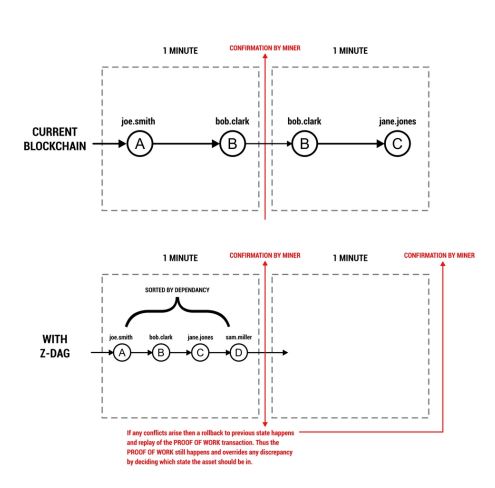
\includegraphics[width=3in]{img/current_vs_zdag.png}
\caption{Current Blockchain design vs Z-DAG 当前的区块链设计vs Z-DAG} 
\label{fig:current_vs_zdag}
\end{figure} 

Figure \ref{fig:current_vs_zdag}  shows the difference between a regular blockchain and Syscoin’s Z-DAG implementation. Syscoin now has two consensus layers. The upper layer consists of a Z-DAG graph of transactions are represented in the mempool without a block, providing settlement in real-time. The lower layer provides confirmation and conflict resolution preventing double-spend events through existing Proof-of-Work (PoW) consensus. 图1展示了常规区块链和Syscoin的Z-DAG之间的区别。目前,Syscoin有两个共识层:第一层中,在不含区块的内存池(mempool)中展示交易的Z-DAG图,提供实时结算。第二层通过现有的工作量证明共识进行确认并提供冲突解决方案,以防止双重支出问题。

When verifying, client nodes will create a graph of transactions topologically arranged via ascendants and descendants organized by the asset UTXO being spent. This is the most efficient approach as a circuit detection is not required; rather, it is inherently assumed as it is added to coin indexes in the memory pool. 验证时,客户端节点将创建一个交易图,通过已花费的资产UTXO 规划的先后,对这些交易进行拓扑排列。这是最有效的途径,因为无需电路检测;更确切的说,当它被添加到内存池中的硬币索引时,本质上也仅仅是假设。

Z-DAG is a transactional algorithm and does not affect consensus policy. It is meant to be a double-spend detection and prevention algorithm through the transaction policies of Syscoin Core. Z-DAG 是一种交易算法,不影响共识策略,目的在于通过 Syscoin Core的交易策略成为一种双重支出检测和预防算法。

A User Interface (UI) layer will notify the user of conflicts in real-time, allowing the transaction to occur in 3 to 5 seconds (i.e., the amount of time the network takes to notice that 2 double-spend transactions are conflicting with each other). This is possible through Syscoin’s Masternode layer that consists of incentivized full nodes paid an allocation of subsidy every block. Every masternode is connected to 25 or more peers, which facilitates high-throughput relay across the network, averaging one or more network hops to transmit from the sender to the receiver nodes. A 用户界面 (UI) 层将实时通知用户冲突,允许交易在3 -5秒之间发生(即网络注意到2个双重支出交易彼此冲突的时间)。这可以通过Syscoin的主节点奖励计划(Masternode)层实现,该层由激励的全节点组成,每个区块都支付补贴。每个Masternode连接到25个或更多的点,这些点在网络中提供高吞吐量的转播,将一个或多个网络跳数均衡从发送方传输到接收方节点。

To accurately detect double-spends, other implementations such as Phantom \cite{Som18} or Spectre \cite{Som15} must replace the longest chain rule to derive the order of events and attacker sequences in a graph.
These implementations end up in a more complex game theoretical situation that has not  been proven mathematically to be accurate in all cases. Syscoin relies on the thoroughly tested Nakamoto consensus model to arrive at a consensus over time rather than simply relying on a DAG. 为精准地检测出双重支出,其他的实施方案如Phantom [6] or Spectre [5]必须替换最长链规则,以推算出图表中事件和攻击者的顺序。最终这些实施方案会形成一个更复杂的、尚未从数学上证明所有情形都正确的博弈论。Syscoin并非仅仅依赖于一个DAG,而是凭借已全面测试的Nakamoto共识模型,以期逐渐达成共识。

\subsection{Order-of-events preservation and Conflict Resolution 事件保存及冲突解决的顺序}
Since assets have been migrated to a UTXO model in Syscoin 4, order-of-events and conflict resolution is as simple as relying on the existing UTXO policy of the Bitcoin memory pool code, which orders individual UTXO dependencies as ascendants and descendants per output. The conflict resolution code for double-spending an output was slightly adjusted from the Bitcoin policy by allowing one double-spend attempt for each output to propagate across the network. This ensures that a double-spend will always be detectable by an observer regardless of order-of-events. This is especially important as nodes on the network have no ability to understand the intent of a transaction and are thus not able to know which one is actually a double-spend attempt. To account for the extra bandwidth requirements of allowing a double-spend to be propagated, the minimum relay fee paid in the transaction is double that of a regular transaction. 由于资产已迁移到 Syscoin 4 中的 UTXO 模型,事件顺序和冲突解决就像依赖比特币内存池代码的现有 UTXO 策略一样简单,该策略将单个 UTXO 依赖项排序为每个输出的祖先和子孙。 通过允许对每个输出进行一次在整个网络中传播的双重支付尝试,从比特币政策中对双重支付的冲突解决代码进行微调。这确保了不管事件顺序如何,观察者始终可以检测到双重支付。 这一点尤其重要,因为网络上的节点无法理解交易的意图,因而也无法弄清究竟哪个才是双重支付尝试。考虑到允许传播双重支付需要额外带宽,交易中所需支付的最低中继费用是常规交易的两倍。

\subsection{CAP Theorem 定理}
The CAP theorem \cite{Bre12} states that it is impossible for a distributed data store to simultaneously provide more than two out of the following three guarantees: consistency, availability or partition tolerance. Bitcoin attempts to provide a guarantee that transactions are settled, but is not able to do so according to theory. Z-DAG partially trades consistency for availability. Since it is unlikely that a double-spend or re-organization will change the state of someone’s balance, we do not wait for settlement finality by waiting for blocks to confirm. This drastically increases the usability in point-of-sale applications. CAP定理[8]指出,分布式数据存储不可能同时提供如下三种保证中的两种以上:一致性、可用性或分区容错性。比特币试图提供一个交易已结算的凭证,但从理论上来看这是无法完成的。Z-DAG用可用性交换一致性。由于双重支出或重组不会改变人们的余额,我们无需等区块确认最终结算。这就极大地增加了POS应用程序的可用性。

The allowance of instant settlements and increased availability requires paying additional attention to users simply trying to double-spend or send transactions too quickly, which may cause the miner view to change from the general network view. The DAG will order the dependency graph of transactions and process in sequence, allowing for better availability (i.e., client making a request for data gets a response) when it comes to instant state changes. The same CAP constraints as PoW will provide a more responsive money transfer mechanism that may be used as a transaction processor instead of simply a settlement layer. 允许即时结算、提高可用性需要对一些用户进行额外的关注,因为这些用户仅仅只是尝试双重支出或发送交易过快,可能会导致矿工视图从一般网络视图改变。DAG将按序排列交易和进程的依赖关系图,以便在即时状态变化时达到更好的可用性(即,客户端请求数据得到响应)。CAP约束与工作量证明(PoW)相同,将提供一个更具响应性的资金转账机制,该机制可用作交易处理器,而非仅仅是一个清算层。

\subsection{Point-of-sale applications POS应用程序}
The combination of using assets with Z-DAG will allow for point-of-sale applications, providing real-time exchange of cryptocurrency assets/tokens. 资产和Z-DAG的组合将允许使用POS应用程序,为加密货币资产/代币提供实时交换

\subsection{Assets 资产}
We have created a coloured-coin implementation of a UTXO asset model where the commitment to the specific values of the assets are embedded in OPRETURN data carrying payload. The UTXO itself is part of the transaction to keep compatibility with the Bitcoin transaction format. The consensus to prove validity of an asset transaction is to simply compare the map of inputs (pairing of asset GUID and total value across all inputs) and the map of all outputs (pairing of asset GUID and total value across all outputs), which must be equal (note: there is no fee on assets so equality is sufficient to ensure validity). The coin database storing the unspent outputs adds a value to represent the asset identifier (GUID) for asset outputs. 我们创建了一个 UTXO 资产模型的彩色币执行器,对资产特定价值的承诺嵌入在携带有效载荷的 OPRETURN 数据中。 UTXO本身是交易的一部分,以保持与比特币交易格式的兼容性。达成证明资产交易有效性的共识,仅需比较输入映射(资产 GUID 和所有输入的总价值的配对)和所有输出的映射(资产GUID 和所有输出的总价值的配对),尤其应确保平等性(注意:资产不收费,因此平等性足以确保有效性)。在用以存储未花费输出的硬币数据库添加一个数值,来表示资产输出的资产标识符 (GUID)。

\subsection{Non-Fungible Tokens 非同质化代币}

Non-Fungible Tokens (NFTs) are unique Syscoin-based digital assets.  Some potential use cases include: gaming, digital art, physical assets, and digital collectibles. The advantages of using Syscoin over other platforms include, but is not limited to scalability, divisibility, efficiency, and notary capabilities. 非同质化代币(NFT) 是独一无二基于Syscoin的数字资产。一些潜在的实际用例如:游戏、数字艺术、实物资产和数字收藏品。与其他平台相比,使用 Syscoin 的优势包括但不限于可扩展性、可分割性、效率和公证能力。

By utilizing the NEVM, Syscoin will offer NFTs running on the application layer of its tech-stack, which will offer a competitive advantage over Ethereum in terms of scalability. Another interesting feature Syscoin will offer is divisibility. A good example of this is land ownership where fractions of such assets can be apportioned between multiple parties. Finally, developers will be able to employ notary capabilities by applying custom rule sets to transactions involving NFTs. 通过应用NEVM,Syscoin 将提供在其技术堆栈的应用层上运行的NFT,NFT在可扩展性方面竞争优势优于以太坊。 Syscoin提供的另一个有趣的功能是可分割性。土地所有权就是一个很好的例子,这种资产的一部分可以在多方之间分配。 最后,通过将自定义规则集应用于涉及 NFT 的交易,开发者将能够使用公证功能。

NFT, fractional or otherwise, are implemented in the UTXO asset model and of course can be deployed using the ERC-related specifications on the NEVM model as is the case with Ethereum. Notary capabilities are only implemented for the UTXO asset model. However, with validity proofs we are looking to integrate such features on the NEVM model as well. NFT以一部分的形式或以其他方式在 UTXO 资产模型中实现,当然可以像以太坊一样使用NEVM模型上的ERC相关规范进行部署。公证能力仅适用于 UTXO 资产模型。 通过有效性证明,我们希望在 NEVM 模型上也可以集成这些功能。

\subsection{Decentralized Identity 去中心化身份}
Decentralized Identity is the cornerstone for secure information and value exchange between people and devices. Typically current implementations leverage Hyperledger Aries to build Identity solutions following the Web3 RFC spec for Decentralized Identifiers (DID's) \cite{DID}. Through the use of public permission settlement of state, and zero-knowledge-proof based validity proofs to attest identity information (i.e., birth certificate or college diploma), we believe this is an ideal solution, which will not only scale to multiple jurisdictions needing to rely on identities issues by governments, but also allow for applications utilizing  social proof-of-person. Scaling is a challenge not only for privacy chains but also private-permissioned blockchains (the registrations of identities are not aggregated and put onto the ledger on a FIFO basis) There is also the issue that settlement happens not on public infrastructure but private and so is susceptible to attacks, which casts doubts over the claim of immutability. Built on zkRollup infrastructure, identity systems can not only scale, but data can remain private and settlement of state can be done on public infrastructure. We leave specific implementations up to integrators and enterprises looking to build next-generation identity solutions. 去中心化身份是人与设备之间交换安全信息和价值的基石。当前的通常方式是利用 Hyperledger Aries 为去中心化标识符 (DID) [53] 构建符合 Web3 RFC 规范的身份解决方案。通过使用状态的公共许可结算 通过使用公共许可的状态结算,以及基于零知识证明的有效性证明来证明身份信息(即出生证明或大学文凭),我们相信这是一种非常理想的解决方案,不仅可以扩展到需要依赖政府身份问题的多个司法管辖区,同时也可以利用社会身份证明的应用程序。不管是对于隐私链还是私有许可的区块链而言,扩展都是一个挑战(注册身份未在FIFO的基础上聚合并放在分类账上)。还有个问题是,结算不是在公共基础设施上而是在私人基础设施上进行的,因此容易受到攻击,这使得其不变性的主张令人质疑。身份系统建立在 zkRollup 基础设施之上,不仅可以扩展,数据还可以保持私有,状态的结算可以在公共基础设施上完成。我们将具体实施方法留给希望构建下一代身份解决方案的集成商和企业。

\subsubsection{Selfish mining 自私挖矿}

Selfish mining is a long standing open problem in the Bitcoin ecosystem \cite{Eya18}. However, with the introduction of masternodes and the ChainLocks service, we have innovated a mechanism design that falls back to Nakamoto consensus. Yet, if a chain lock in a block exists will remove selfish mining attack vectors. To understand the solution it is important to understand the design of Multi-quorum based Chain locks. 自私挖矿是比特币生态系统中一个长期存在悬而未决的问题 [11]。 但随着masternodes(主节点)和ChainLocks(链锁)服务的引入,我们创新了一种退回到中本聪共识的机制设计。如果区块中存在链锁,则会消除自私挖矿攻击向量。如需了解解决方案,则应先弄清基于Multi-quorum的链锁的设计。

\subsubsection{Chain locks 链锁}

With a subset of nodes offering sybil resistance through the requirement of bonding 100,000 SYS to become active, along with the deterministic masternode feature added in Syscoin 4.2, we have enabled Chain Locks to prevent selfish mining. Dashcore was the first project to implement this idea \cite{Blo18}, which the industry has since widely accepted as a viable solution \cite{Val19}. Our implementation is a simplified and optimized version of the original. We do not implement Instant Send or Private Send transactions. Due to Syscoin being merged-mined with Bitcoin, we believe our chain coupled with Chain Locks becomes more secure via solving Bitcoin’s most vulnerable attack vector (i.e., selfish mining). 通过要求绑定100,000个SYS才能激活的节点子集提供女巫防御,以及在 Syscoin 4.2 中添加的确定性主节点功能,我们启用了链锁以防止自私挖矿。 Dashcore是首个将该想法付诸现实的项目 [22],业界已广泛接受其作为可行的解决方案 [18]。 相比于原始版本,我们的实施方式更加简化和优化。 我们不实施即时发送或私人发送交易。 由于 Syscoin 与比特币联合挖矿,我们认为通过解决比特币最脆弱的攻击向量(即自私挖矿),链与链锁相结合会变得更加安全。

Chain Locks are made part of Long-Living Quorums (LLMQ) which leverage aggregatable Boneh–Lynn–Shacham (BLS) signatures that have the property of being able to combine multiple signers in a Distributed Key Generation (DKG) event to sign on decisions. In this setup, a signature can be signed on a group of parties under threshold constraints without any one of those parties holding the private key associated with that signature. In our case, the signed messages would be a ChainLock Signature (CLSIG) which represent claims on what block hashes represent on the canonical chain \cite{Blo18}. This model suggests a very efficient   threshold signature design was needed to reach consensus across the Masternode layer, decide on chain tips, and lock chains, hence preventing selfish mining attacks. See \cite{Bon18} to understand the qualities of BLS signatures in the context of multi-signature use cases. 链锁是长效仲裁 (LLMQ) 的一部分,它利用可聚合的 Boneh-Lynn-Shacham (BLS) 签名算法,该签名具有以下特性:能够在分布式密钥生成 (DKG) 事件中组合多个签名者以签署决策。在此设置中,可以在阈值约束下,由一组参与方签署签名,(一组参与方可以签署出一个签名,)这些参与方中的任何一方都不持有与该签名相关联的私钥。在我们的案例中,签名的消息将是一个链锁签名(CLSIG),它代表了区块哈希在规范链上所代表的声明内容 [22]。 该模型表明需要一个非常有效的阈值签名设计以在主节点层达成共识、决定链提示和锁定链,从而防止自私挖矿攻击。如需了解多签名用例上下文中的BLS 签名特质,请参见 [19] 。

Ethereum 2.0 caters to the use of BLS signatures through adding precompile opcodes in the Ethereum Virtual Machine (EVM) for the BLS12-381 curve \cite{Dra18}, which Syscoin has adopted. This curve was first introduced in 2017 by Bowe \cite{Bow17}  to the ZCash protocol. Masternodes on Syscoin have adopted this curve and have a BLS key that is associated with each validator. See \cite{Blo18} for performance comparison to ECDSA (Secp256k1) and a discussion on usefulness in contrast to what Bitcoin and Syscoin natively use for signature verification. Ethereum 2.0 通过在以太坊虚拟机 (EVM) 中为 BLS12-381 曲线 [20](Syscoin 已采用该曲线)添加预编译操作码,从而满足BLS 签名的使用。 该曲线于 2017 年由 Bowe [21] 首次引入 ZCash 协议。 Syscoin主节点采用了此曲线,并具有与每个验证器关联的 BLS 密钥。 关于与 ECDSA (Secp256k1) 的性能比较以及与比特币和 Syscoin 本身用于签名验证的对比的有用性的讨论,请参见 [22]。

\subsection{Lightning Networks 闪电网络}
By extending on the UTXO asset model we look to integrate layer 1 assets into transactions on layer 2 payment channels such as Lightning Networks \cite{Poon16}. Adding multiple assets to LN requires solving theoretical attack vectors related to American call-options as described in \cite{LN}. Since Syscoin UTXO assets enable the transacting of multiple assets in a single transaction, the integration into Lightning Networks should be fairly intuitive once the problems related to American call-options are solved for. 通过扩展 UTXO 资产模型,我们希望将第1层资产集成到第2层支付渠道(如闪电网络 [54])上的交易中。如需将多个资产添加到闪电网络,则需解决与美式看涨期权相关的理论攻击向量,如 [55] 所述。 由于 Syscoin UTXO 资产能够在单笔交易中处理多种资产,一旦解决了美式看涨期权相关的问题,集成到闪电网络将会相当直观。

\subsection{Masternodes 主节点}

With 2500+ current, active masternodes running fullnodes, Z-DAG becomes more dependable, as does the propagation of blocks and potential forks. Masternodes are bonded through a loss-less strategy of putting 100,000 syscoin in an output and running full nodes in exchange for block rewards. A seniority model incentivizes masternodes to share long-term growth by paying more for the longer period of service as an additional incentive. Half of the transaction fees are shared between the PoW miners and masternodes to ensure long-term alignment once block subsidy becomes negligible. Coins are not locked at any point, and there is no slashing condition if masternode owners decide to move their coins, the rewards to those masternodes simply stop. Sharing Bitcoin’s compact block design, it consumes very little bandwidth to propagate blocks assuming the memory pool of all these nodes is roughly synchronized \cite{BitCore}. The traffic on the network primarily consists of propagating the missing transactions to validate these blocks. Having a baseline for a large number of full nodes that are paid to be running allows us to create a very secure environment for users. It proposes higher costs to would-be attackers who either have to attempt a 51\% attack on Syscoin (i.e., effectively trying to attack the Bitcoin network), or try to game the mesh network by propagating bad information which is made more difficult by incentivized full nodes. The health of a decentralized network relies on the following; (a) the mining component, or consensus to produce blocks, and (b) the network topology to disseminate information in a timely manner in conditions where adversaries might be lurking. The likelihood of other attacks related to race conditions in networking or consensus code are minimized by following a rigorous, thorough and continuous development process. This includes deterministic builds, Fuzz tests, ASAN/MSAN/TSAN, functional/unit tests, multiple clients and adequate code coverage. Syscoin and Bitcoin protocol code bases are merged daily such that the build/signing/test processes are all identical, allowing us to leverage the massive developer base of Bitcoin.  Code quality is reflective of taking worst-case situations into account. 拥有2500多个当前运行全节点的活跃主节点,Z-DAG变得愈加可靠,区块和潜在分叉的传播亦是如此。通过以下无损策略对主节点进行绑定:将 100,000个Syscoin放入输出并运行完整节点以换取区块奖励。资历模型激励主节点通过为更长的服务期限支付更多费用作为额外奖励来分享长期增长。PoW 矿工和主节点共享一半的交易费用,以防止一旦区块补贴变得可以忽略不计,还可确保长期联盟。 代币在任何时候都不会被锁定,如果主节点所有者决定移动他们的代币,则没有削减条件,对这些主节点的奖励会直接停止。共享比特币的致密区块设计,假设所有这些节点的内存池大致同步,则传播区块所消耗的带宽随之变少 [16]。 网络上的流量主要用于传播丢失的交易以验证这些区块。我们拥有大量付费运行的完整节点作为基线,能够为用户创建一个非常安全的环境。这种方式需要潜在攻击者付出更高成本,他们要么需要尝试对 Syscoin 进行 51\% 的攻击(即,尝试有效攻击比特币网络),要么尝试通过传播不良信息来操纵网状网络,而激励全节点使之难上加难。去中心化网络的健康取决于: (a) 挖矿组件,或产生区块的共识, (b) 在对手可能潜伏的情况下能够及时传播信息的网络拓扑。在网络或共识代码中,可以通过遵循严格、彻底和持续的开发过程,将与竞争条件相关的其他攻击的可能性降到最低。这包括确定性构建、模糊测试、ASAN/MSAN/TSAN、功能/单元测试、多个客户端和足够的代码覆盖率。 Syscoin 和比特币协议代码库日常合并,这样构建/签名/测试过程都是相同的,以便我们能够充分利用比特币的庞大开发人员库。代码质量反映了将最坏情况纳入考虑范围之中。

\section{Roadmap to Web 3.0 网络路线图3.0}
\label{section:roadmap}

Bitcoin was the first to offer a practical solution to the General's Dilemma using Crypto Economic rationale and incentives. Ethereum was the first to abstract the concept of Turing completeness within similar frameworks assumed by Bitcoin. What Syscoin presents is a combination of both Bitcoin and Ethereum with intuitions built on top to achieve a more efficient financial computing platform that leverages coordination to achieve consensus using Crypto Economic rationale and incentives. We propose a four-layer tech stack using Syscoin as the base (host) layer, which provides an efficient (i.e., low gas cost per transaction) platform. Some of the main advantages include scalable, decentralized enabling applications, and the introduction of a decentralized cost model around Ethereum gas fees. This new model proposes state-less parallelized execution and verification models while taking advantage of the security offered by the Bitcoin protocol. 比特币首次实现通过加密经济原理和激励措施为将军困境提供实用解决方案。以太坊首次实现在比特币假设的类似框架内将图灵完备性概念提取出来。而Syscoin呈现的是比特币和以太坊的直观结合,以建立更高效的金融计算平台,该平台通过协调加密经济原理和激励机制来达成共识。我们提出了一个使用 Syscoin 作为基础(主机)层的四层技术堆栈,提供了高效(即每笔交易低gas cost)平台。主要优势包括可扩展的、去中心化启用应用程序,以及围绕以太坊gas cost引入去中心化成本模型。这种新模型提出了无状态并行执行和验证模型,同时充分利用比特币协议所提供的安全性。

\subsection{Scalability and Security 可扩展性和安全性}

Scalability in blockchain environments is typically measured by total Transactions per Second (TPS). This suggests full trustlessness, decentralization and liveness properties as evidenced by something like Bitcoin. If trade-offs are made to achieve higher scale, it means another property is affected. If two nodes are running the same hardware and doing the same work, the one that provides more TPS performance than the other is considered more scalable. This is not to be confused with throughput which is the measure of output that can be increased by simply adding more hardware resources. Hence, more throughput does not mean more scalable. Some blockchains require the producers of blocks to run on higher specifications, thus offering higher throughput but not necessarily scaling better. However, there are projects which employ parallel processing to try to achieve higher scale whilst also enforcing more capable hardware to provide a more efficient overall system [33]. As a logical experiment, the throughput of a system divided by the scalability of the system is what we define as efficiency. In the following sections, we will outline our proposal for improved efficiency. 通常,区块链环境中的可扩展性通过每秒总交易数 (TPS) 来衡量。正如比特币所证明的那样,这表明了完全的去信任、去中心化和活跃的特性。如果为了实现更高的规模而进行交易,则意味着另一个属性会受到影响。如果两个节点运行相同的硬件、执行相同的工作,那么TPS 性能更高的那个节点则被认为更具可扩展性。但请不要将它与吞吐量混淆,吞吐量是可以通过简单地添加更多硬件资源来增加的输出量度。由此,吞吐量更高并不意味着可扩展性更大。一些区块链要求区块的生产者以更高的规格运行,以求提供更高的吞吐量,而不求更好地扩展。然而,有些项目采用并行处理的方式,试图实现更高的规模,同时还采用更强大的硬件以提供更高效的整体系统 [33]。作为一个逻辑实验,系统的吞吐量除以系统的可扩展性就是我们所定义的效率。在下文中,我们将概述关于如何提高效率的建议。

\subsubsection{Efficiency 效率}

The holy grail of blockchain design resides in the ability to have a ledger that can claim to be sublinear while retaining consistency, fault tolerance, and full availability (i.e., CAP Theorem). Hence, there are roughly constant costs for an arbitrary amount of computation performed and being secured by that ledger. Achieving this optimal tradeoff has always been thought of as impossible, unless acceptable trade-offs appear in application designs that are easy to understand. Most experts make the assumption that an O(1) ledger is simply impossible and thus design blockchains, and force applications, to work in particular ways as a result. We will remove such assumptions and let business processes dictate how they work by giving them the ability to achieve O(log kn) efficiency with trade-offs. A polylogarithmic design would give the ability for almost infinite scaling over time for all intents and purposes. The only bottleneck is the speed at which information can be propagated across the network. This in turn would improve over time as telecom infrastructure naturally evolves and increases in both capability and affordability. 区块链设计的圣杯在于能够拥有一个可以声称是次线性的分类帐(ledger),与此同时还可以保持一致性、容错性和完全可用性(即 CAP 定理)。因此,执行任意数量的计算并由该分类账保护,其成本大致恒定。除非在易于理解的应用程序设计中出现可接受的权衡,否则没人会相信达到最佳权衡。大多数专家假设 O(1) 分类账根本不可能,因此设计区块链并强制应用程序以特定方式工作。我们将消除此类假设,并让业务流程通过权衡实现O(log kn) 效率的能力来决定它们的工作方式。多对数设计可以为所有意图和目的提供可随时间几乎无限扩展的能力。唯一的瓶颈在于信息在网络中传播的速度。随着电信基础设施的自然发展、能力和可负担性的提高,这种情况也会随着时间的推移而改善。

Put in context, even Lightning Networks qualifies for transactional counts qualifies as a form of sublinear scaling on a TPS basis, but not per user as users must enter the main chain first before entering a payment channel. It requires the state of the blockchain to include users joining the system. This state (i.e., UTXO balances) is the primary  factor of efficiency degradation in Bitcoin. Users need to first start on the main chain and then move into the payment channel system to receive money, meaning that scale is at best O(N) where N is the number of users. There are some solutions to the problem of state storage on Bitcoin \cite{Dry19} (e.g., by reducing it via an alternative accumulator strategy to the cost of increased bandwidth). This approach would make the chain state-less. However, validation costs would remain linear in the number of transactions. When combined with payment channels, only costs to get in/out are factored into the validation. This offers an interesting design for payments themselves while providing for on-chain availability to help achieve scalable payments. Hence, it is not possible to employ that strategy with general computations. With this design we are still left with the issue of how to do general computations at higher efficiency. 在上下文中,即使闪电网络有资格获得交易计数,也有资格作为基于 TPS 的一种次线性扩展形式,但并不惠及每个用户,因为用户必须先进入主链,然后才能进入支付渠道。它要求区块链的状态将入驻系统的用户包含在内。这种状态(即 UTXO 余额)是比特币效率下降的主要因素。用户需要首先在主链上启动,然后进入支付渠道系统接收资金,这意味着规模最多为 O(N),其中 N 是用户数量。关于比特币 [27] 的状态存储问题有一些解决方案(例如,通过使用替代累加器策略来减少日益增多的带宽成本)。这种方法将使链无状态。但是,验证成本将与交易数量保持线性关系。当与支付渠道结合时,只有进入/退出的成本会被纳入验证。这为支付本身提供了一个饶有趣味的设计,同时提供了链上可用性以帮助实现可扩展的支付。因此,一般计算中不可能使用该策略。如使用该设计,我们仍将面临这样的问题:怎样以更高的效率进行一般计算?

What we present is the ability to have a polylogarithmic chain at the cost of availability for both payments and general computations, where business processes dictate availability policies and users fully understand the limitations of these policies when using such systems. Users will ensure availability for themselves and others at their discretion.  This will be expanded upon in the following sections. 我们所展现的是能够以支付和一般计算的可用性为成本,从而获得多对数链的能力,其中业务流程规定了可用性策略,用户在使用此类系统时完全理解这些策略的局限性。用户将自行决定确保自己和他人的可用性。下文中将对此进行扩展。

\subsubsection{State Liveness and State Safety 状态活跃性和状态安全}

While many compelling arguments can be made migrating to a stateless design \cite{Hot19}, it is not possible to achieve sublinear efficiency without sacrificing some other desired component as outlined above. To achieve polylogarithmic efficiency, it is necessary to have a mix of stateless and stateless nodes working together in harmony on a shared ledger \cite{Hot19}. This should be accomplished so that business processes can dictate direction and users can choose to pay a little more for security, either by using a stateful (yet very scalable ledgering mechanism) or by paying to ensure their own data availability amortized over the life of that user on such systems. Presenting the ability for users to make these choices allows us to separate the consensus mechanism of such systems and reduce overall complexity. However, in whatever solution we adopt, we need to ensure that the final implementation allows for both the liveness and safety of that state. These are defined as follows:

\begin{itemize}
\item \textbf{State Liveness}: Transferring coins in a timely manner
\item \textbf{State Safety}:  Private custody
\end{itemize}

虽然可以将许多令人信服的论点迁移到无状态设计 [28],但如果不牺牲上述一些其他所需的组件,则不可能实现次线性效率。为了实现多对数效率,有必要让无状态和无状态节点在共享账本上和谐一致、协同工作 [28]。应该实现这些想法,以便业务流程可以指示方向,并且用户可以选择为安全性多支付一些费用,或者通过使用有状态(但非常可扩展)的分类账机制,或者通过付费以确保此类系统上的用户的数据可用性在生命周期内摊销。为用户提供选择的能力,使我们能够分离此类系统的共识机制并降低整体复杂性。然而,无论我们采用何种解决方案,我们都需要确保最终的实现方式能够允许该状态的活跃度和安全性并存。具体定义如下:

\begin{itemize}
\item \textbf{状态活跃度}: 及时转移币
\item \textbf{状态安全性}: 私人保管
\end{itemize}

It is important to adhere to these concepts; unmoveable coins are worthless. 遵从这些概念很重要;无法转移的币毫无价值。

The options as described would allow users to decide their state liveliness at their own discretion, while state safety is a required constraint throughout any system design we provide. The doorway to possibilities of sublinear design is opened by giving users the ability to decide. 上述选择将允许用户自行决定他们的状态活跃度,而状态安全性是我们提供的任何系统设计中的必需约束。通过让用户自主决定,打开了可能通往次线性设计的大门。


\subsubsection{Avoiding Re-execution of Transactions 避免重新执行交易}

In order to scale arbitrarily, and independently of the number of transactions (a desired property of increasing throughput), one requires a mechanism to avoid re-executing transactions \cite{Bow18}; as these transactions put unnecessary additional overhead on the network. Ideally, it would be able to batch these transactions together for a two-fold scaling proposition. There are a few mechanisms in literature that attempted to solve re-execution: (a) TrueBit; (b) Plasma; and (c) Arbitrum avoided re-execution. Unfortunately, they require challenge response systems to ensure security, which leads to intricate attack vectors of unbounded risk/reward scenarios.  为了任意扩展且独立于交易数量(吞吐量增加的理想特性),人们需要一种机制避免重新执行交易 [29]; 因为这些交易给网络带来了不必要的额外开销。理想状态下,这些交易可以一批次处理,以实现双重扩展。文献中有一些试图解决重新执行的机制: (a) TrueBit; (b) Plasma; (c) Arbitrum 避免重新执行。但非常不幸的是,这些机制需要挑战响应系统来确保安全性,这会引起无限风险/回报场景的复杂攻击向量。

Multi-Party Computation (MPC) is a mechanism that allows for shared computation while maintaining confidentiality and privacy. MPC is used in Syscoin for BLS threshold signatures for Chain Locks and Proof-of-Service in quorums of validators, deterministically chosen using Fiat-Shamir heuristics on recent block hashes. The problem with this approach is that validators may become corrupt, hence they need to be wrapped in a consensus system along with distributed key generation (DKG) and random deterministic selection. It was discarded due to the incentive for risk/reward scenarios to favour attacks as the value of the transactions increases. 安全多方计算 (MPC) 是一种允许共享计算的同时还可保持机密性和隐私的机制。 MPC 在 Syscoin 中用于链锁的 BLS 阈值签名和验证者仲裁中的服务证明,使用 FiatShamir 启发式算法对最新的区块哈希进行确定性选择。这种方式的风险在于验证器可能会损坏,因此它们需要与分布式密钥生成 (DKG) 和随机确定性选择一起打包在共识系统中。随着交易价值的增加,风险/回报场景的激励容易吸引攻击,所以弃之不用。

Hardware enclaves (e.g., Intel SGX through remote attestation) were considered as a way to offload execution and avoid re-execution costs. 硬件飞地(举例,通过远程认证的英特尔 SGX)被认为是一种卸载执行并避免重新执行成本的方法。

ZKP allows for the desired superlinear scaling trait, but also offers other benefits - namely privacy is very easy to introduce and will not add detectable costs or complexity to verification on the mainchain. With users controlling their own data the mainchain and systems can be designed such that only balance adjustments are recorded, not transaction sets (we will explain the case with full data availability below). In this scenario there is no advantage for a miner to gain when colluding with users that launch attacks on systems such as Decentralize Finance (DeFi), pools and provenance of transactions. The flexibility has to be present for application developers that need experiences consistent with those we have today with Bitcoin/Syscoin/Ethereum. This would enable the privacy use-cases without requiring extra work, knowledge or costs. ZKP 允许所需的超线性扩展特性,同时也提供其他好处——即易于启用隐私,并且不会增加可检测的成本或主链验证的复杂性。 通过用户控制自己的数据,主链和系统可以设计成只记录余额调整,而不记录交易集(我们将在下文中解释完整数据可用性的情况)。 在这种情况下,当矿工与用户串通对去中心化金融 (DeFi)、矿池和交易来源等系统发起攻击时,不会获得任何优势。 必须为需要与我们当前在Bitcoin/Syscoin/Ethereum上拥有一致经验的应用程序开发人员提供灵活性。这将启用隐私用例,无需额外的工作、知识或成本。

\subsubsection{Validity Proof Systems 有效性证明系统 Overtop Proof-of-Work Systems 系统}

Prior to the use of Proof Systems, the only option for “Validity Proofs” in a permissionless system involved naive replay, which greatly limited scalability. Essentially, this is still practised in Layer-1 blockchain (L1) solutions, with the known penalty to scalability. Proof Systems offer a very appealing trait known as succinctness. How this works, in order to validate a state transition, one needs to only verify a proof, and this is done at a cost that is effectively independent of the size of the state transition (i.e., polylogarithmic in the size of the state transition). 在使用证明系统之前,无许可系统中“有效性证明”的唯一选择涉及幼稚重放,(单纯的重播)这极大地限制了可扩展性。 从本质而言,这仍然在第 1 层区块链 (L1) 解决方案中实践,显然会损害可扩展性。 证明系统提供了一种非常吸引人的特性- 简洁。这些都是如何运转的?为了验证状态转换,人们只需要验证一个证明,这是以有效独立于状态转换大小的成本完成的(即,状态转换大小的多对数)。

For maximal financial security the amount of value being stored should depend on the amount of security provided on the settlement side of the ledger. PoW offers the highest security guarantees (see Appendix A). Our next generation financial systems begin with optimal ledgering security and add proof systems on top for scaling. Block times are not as important in a world where the majority of activity is on Layer-2 blockchain (L2) validity proof based systems. This liberates engineers, who are focused on scalability, to better define blocks, safe block times, as well as the maximal amount of data bandwidth that can be safely propagated in a time-sensitive manner across full nodes in the network. With Syscoin, there are incentivized full nodes (i.e., deterministic masternodes). So, again we can maximize the bandwidth of ledgering capabilities while retaining Bitcoin PoW security through merged-mining. 为确保最大的财务安全性,存储的价值量应取决于分类账结算端提供的安全量。 PoW 提供最高安全保证(见附录 A)。 我们的下一代金融系统从最佳分类账安全性开始,并在顶部添加证明系统以进行扩展。大多数活动都在基于第2层区块链 (L2) 有效性证明的系统上,在这样的世界里,区块时间并不重要。这就解放了专注于可扩展性的工程师,以更好地定义区块、安全块时间以及可以在网络中的完整节点之间高时效安全传播的最大数据带宽量。 使用 Syscoin意味着拥有激励的全节点(即确定性主节点)。 因此,我们可以再次最大化分类账功能的带宽,同时合并挖矿,以保持比特币 PoW 的安全性。

\subsubsection{Quantum Resistance 量子抵抗}

Hashing with the SHA256 algorithm is regarded to be quantum safe because it requires Grover's algorithm to crack in the post-quantum world, and at best a quantum computer will offer a 50\% reduction in time to break \cite{Nai19}. On the other hand, where Shor’s algorithm applies, any pair based cryptographic system will be broken in hours. 使用 SHA256 算法哈希被认为是量子安全的,因为它要求格罗弗算法在后量子世界中破解,而量子计算机最多可以将破解时间缩短 50\% [34]。 另一方面,在 Shor 算法适用的情况下,任何基于成对的加密系统都将在数小时内被破解。

For L2, we propose to implement ZKP in the SDK Layer; namely Non-Interactive Zero Knowledge Proofs (NIZKP). Popular implementations of NIZKP include Zero-Knowledge Succinct Non-interactive ARgument of Knowledge (zk-SNARKS) and Zero-Knowledge Scalable Transparent ARguments of Knowledge (zk-STARKS) \cite{Nas19}. There are some zk-STARK/zk-SNARK-friendly ciphers employed in zkRollup designs, such as MiMC and Pederson hashes, that would offer quantum resistance within ZKPs. However, we currently lack certainty on their classical security; despite this we are hopeful. 对于L2,我们建议在SDK层实现ZKP; 即非交互式零知识证明(NIZKP)。 NIZKP 的流行实现包括零知识简洁非交互式知识论证(zk-SNARKS)和零知识可扩展知识的透明论证(zk-STARKS)[35]。 在 zkRollup 设计中采用一些 zk-STARK/zk-SNARK 友好加密,如 MiMC 和 Pederson 哈希,它们将在 ZKP 中提供量子抵抗。目前我们无法确定它们的经典安全性能;但尽管如此,我们还是充满希望。

It is essential to acknowledge that Bitcoin was developed with change addresses in mind. Stealing Bitcoin requires exposing the hash of its public key, which can be done using Grover’s algorithm running on a quantum computer. Each time a Bitcoin Unspent Transaction Output (UTXO) is spent the public key is exposed and a new change address (which does not expose the public key) is used as change. 不得不提到的是,开发比特币时考虑到了地址变更。窃取比特币需要公开其公钥的哈希,这可以使用在量子计算机上运行的格罗弗算法来完成。 每次花费比特币未支出交易输出 (UTXO) 时,都会公开公钥,并使用新的找零地址(不公开公钥)作为找零。

With this in mind, any scalable L2 solution should be quantum resistant because otherwise we undermine Bitcoin design as the gold standard of security. 考虑到这一点,任何可扩展的 L2 解决方案都应该是抗量子的,否则我们就是公然挑衅在安全性方面被认为是黄金典范的比特币设计。

\subsection{Design Proposal for Web 3.0 的设计提案}

The following describes the four layers (see Fig 2) of Syscoin’s proposed tech stack for Web 3.0:
以下是Syscoin为 Web 3.0 提出的技术堆栈的四个层级(见图 2):

\begin{enumerate}
\item \textbf{Host Layer 主机层:} Bitcoin’s design is the gold standard for security and decentralization. PoW and Nakamoto Consensus settlement security are widely regarded by academics as the most hardened solution for ledgering value \cite{Bit15}. However, it is also arguable that the intricate design encompassing Game Theory, Economics, risk reward ratios for attack, and the minimal amounts of compromising attack vectors is likely not to change for the foreseeable future. UTXOs (and payments with them) are more efficient than account-based or EVM-based solutions. That said, Bitcoin itself suffers from not being expressive enough to build abstraction for general computation. 比特币的设计是安全和去中心化的黄金标准。 PoW 和 Nakamoto Consensus 结算安全被学术界广泛认为是账本价值的最坚实的解决方案 [14]。 当然也存在一些争议,包括博弈论、经济学、攻击的风险回报比和最小数量的妥协攻击向量在内的复杂设计,在可预见的未来内可能不会改变。 相比较于基于账户或基于 EVM 的解决方案,UTXO(以及使用它们支付)更有效。也就是说,比特币本身的表现力不足以为一般计算构建抽象概念。
\item \textbf{Operating System Layer 操作系统层} EVM/eWASM is the gold standard for general computation because of its wide adoption in the community. Anyone building smart contracts is likely using this model, and will continue to use it as the standard for autonomous general computation with consensus. EVM/eWASM 在社区中广泛应用,是一般计算的黄金标准。 任何构建智能合约的人都可能使用此模型,并将继续将其用作具有共识的自主通用计算的标准。
\item \textbf{SDK Layer SDK 层} Zero-knowledge proofs are the gold standard for generalized computation scaling for blockchain applications. They enable one-time execution via a prover and enable aggregated proof checking instead of re-execution of complex transactions via zk-STARKs or zk-SNARKs using collision resistant hash functions. At the moment generalized smart contracts are not there yet but we are quickly approaching the day (e.g., Cairo, Zinc) when there will be abstractions made to have most Solidity code trans-compile into a native zero-knowledge aware compiler. 零知识证明是区块链应用程序通用计算扩展的黄金标准。它们没有使用抗碰撞哈希函数由zk-STARK 或zk-SNARK重新执行复杂的交易,而是通过一个验证方启用一次性执行,并启用聚合证明检查。目前还不存在通用的智能合约,但这一天指日可待(如,Cairo, Zinc),届时会有抽象概念使大多数 Solidity 代码转编译为原生的零知识感知编译器。
\item \textbf{Application Layer 应用层} Verticals or applications applying the above SDK to define business goals. Verticals or applications采用上述 SDK 来定义业务目标。
应用层 采用上述 SDK的应用方案 来定义业务目标。 
\end{enumerate}

\begin{figure}[h!]
\centering
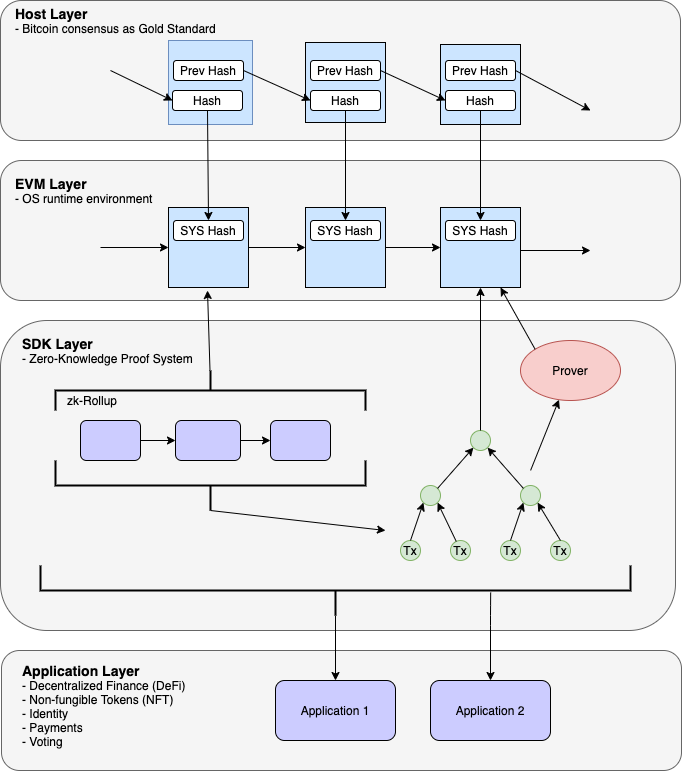
\includegraphics[width=3.5in]{img/4_layer.png}
\label{fig:tech_stack}
\caption{Proposed 4-layer tech stack for Syscoin 为 Syscoin 提议的4层技术堆栈} 
\end{figure} 

Surprisingly, these ideals represent a design that is not shared with any other project in the industry, including Bitcoin or Ethereum. We believe this design, fashioned together in a single protocol, could present a grand vision for a “World Computer” blockchain infrastructure. 令人惊讶的是,这些理想呈现了一种不与业内任何其他项目(包括比特币或以太坊)共享的设计。我们相信这种塑造在一个单一协议中的设计,可以为“世界计算机”区块链基础设施呈现一个宏伟的愿景。

Syscoin has already implemented Geth + Syscoin nodes in one application instance already (i.e., release 4.2). We foresee that there will not be any challenges associated with building a consensus basis working together to form a dual chain secured by Syscoin’s PoW. Syscoin已经在一个应用程序实例中实现了 Geth + Syscoin 节点(即 4.2 版)。 可以预见,通过建立共识基础,在共同努力下可以轻松创建由 Syscoin 的 PoW 保护的双链。

\begin{figure}[h!]
\centering
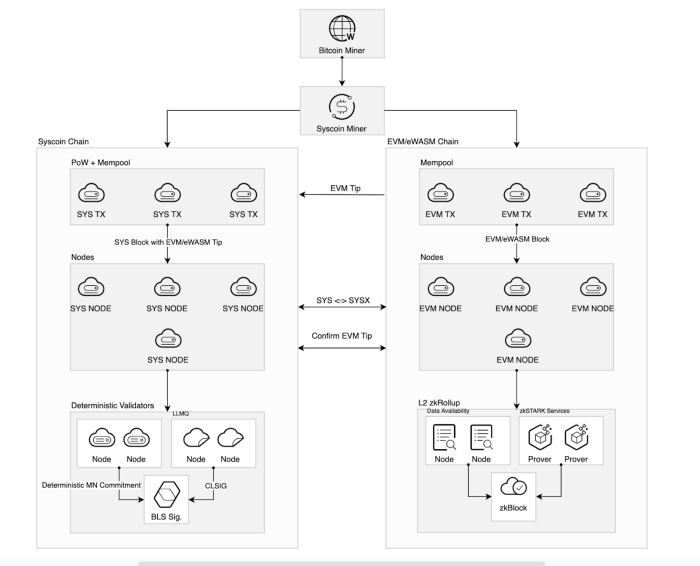
\includegraphics[width=3.4in]{img/fig_5.png}
\label{fig:proposed_design}
\caption{Proposed design 设计建议} 
\end{figure} 

Figure 3 describes a system where nodes are running two sets of software processes, the Syscoin chain protocol and an EVM / eWASM chain protocol which are kept in sync through putting the EVM tip hash into the Syscoin block. Both have their own individual mempools and effectively the Ethereum contracts, tools and processes can directly integrate into the EVM chain. Note that the two chains are processes running on the same computer. Thus a SYS NODE and EVM NODE would be operating together on one machine instance (i.e., full node or masternode) with the ability to communicate with each other directly through Interprocess Communication (IPC). The intersection happens at three points:


\begin{enumerate}
\item Miner of the EVM chain collects the latest block hash and places it into the Syscoin block.
\item When validating Syscoin blocks nodes confirm the validity of the EVM tip by consulting the EVM chain software locally.
\item Fees for the EVM chain are to be paid in SYS. We will enable this through a similar working concept that we’ve already established (SysEthereum Bridge). We may also enable pre-compiles on the NEVM to extract Syscoin block hashes and Merkle roots to confirm validity of SYS to NEVM burn transactions.
\end{enumerate}

主机层-比特币共识作为黄金标准图3所描述的系统,一个节点运行两组软件进程,Syscoin 链协议和 EVM / eWASM 链协议,它们通过将 EVM 提示哈希放入 Syscoin 区块来保持同步。 两者都有自己的独立内存池,并且以太坊合约、工具和流程可以直接有效集成到 EVM链中。需要注意的是,这两个链是在同一台计算机上运行的进程。 因此,SYS 节点和 EVM 节点将在一个机器实例(即完整节点或主节点)上一起运行,并能够通过进程间通信 (IPC) 直接相互通信。 交互发生在三个点:

\begin{enumerate}
\item EVM 链的矿工收集最新的区块哈希并将其放入 Syscoin 区块。
\item 在验证 Syscoin区块节点时,通过本地查询 EVM 链软件来确认EVM提示的有效性
\item EVM 链费用将在 SYS 中支付。我们将通过已建立的类似工作概念(SysEthereum桥)来实现。我们还能够在 NEVM 上启用预编译以提取 Syscoin 区块哈希和 Merkle根,从而确认 SYS 对 NEVM 销毁交易的有效性。
\end{enumerate}

\begin{figure}[h!]
\centering
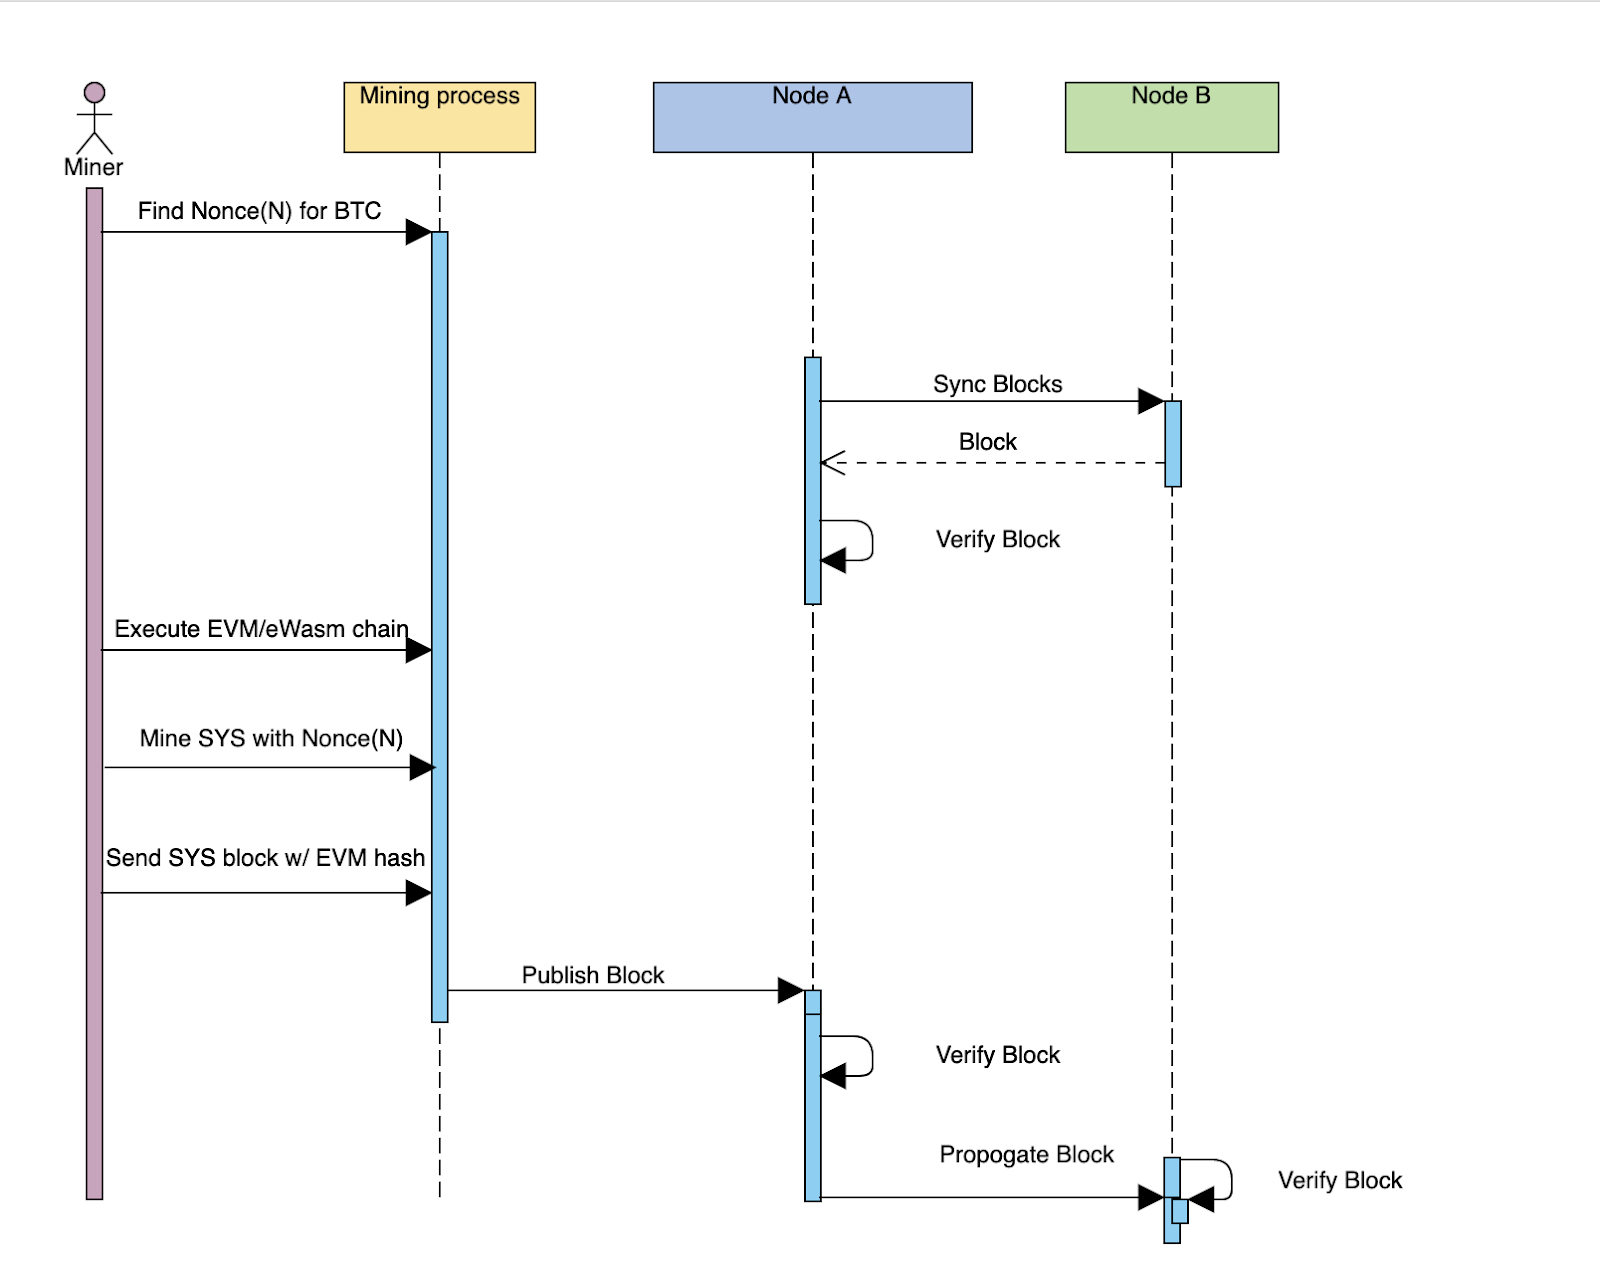
\includegraphics[width=3.4in]{img/fig_6.png}
\label{fig:tech_stack}
\caption{Merge mining on Syscoin Syscoin 上的合并挖矿} 
\end{figure} 

As seen in Figure 4, work done on BTC is reused to create SYS blocks through the merged-mining specification. Concurrently, the miner will execute smart contracts in the memory pool of the node running the EVM chain. Once a chain hash has been established post-execution, it will be put into a Syscoin block and published to the network. Upon receiving these blocks, every node would verify that the EVM chain, which can be locally executed (i.e., same as the miner), matches the state described by the Syscoin block. Technically, one would want to ensure both the latest and previous EVM block hashes inside of their respective Syscoin blocks are valid. The block $->$ evmblock $==$ evmblock \&\& block $->$ prev $==$ evmblock $->$ prev is all that is needed to link the chains together with work done by Bitcoin which is propagated to Syscoin through AUXPOW and can serve as a secure ledgering mechanism for the EVM chain. 如图4所示,重新使用BTC上完成的工作,从而通过合并挖掘规范创建SYS区块。同时,矿工将在运行 EVM 链的节点的内存池中执行智能合约。一旦在执行后链哈希创建完成,它将被放入 Syscoin区块并发布到网络。收到这些区块后,每个节点都会验证可在本地执行(即与矿工相同)的 EVM 链是否与 Syscoin 区块描述的状态相匹配。从技术层面而言,人们希望确保其各自 Syscoin区块内最新和先前的EVM区块哈希都是有效的。 block - > evmblock == evmblock && block - > prev == evmblock - > prev 这是将链与比特币完成的工作链接在一起所需的全部内容,比特币通过AUXPOW传播到Syscoin,并且可以作为EVM 链的安全分类账机制。

Since (a) we may use eWASM; (b) there are paid full nodes running on the network; and (c) the mining costs are shared with Bitcoin miners, we should, therefore, be able to safely increase the amount of bandwidth available in the EVM chain while remaining secure from large uncle orphan rates. There has been much discussion as to what the safe block size should be on Ethereum. Gas limits are increasing as optimizations are made on the Ethereum network. However, since this network would be ledgered by the Syscoin chain through PoW, there should be no concern for uncle orphaning of blocks since the blocks must adhere to the policy set inside of the Syscoin block. We should therefore be able to increase bandwidth significantly and parameterize for a system that will scale globally yet still be centered around L2 rollup designs. In contrast to our design, Ethereum 2.0 centers around a Beacon chain and sharding served by a Casper consensus algorithm \cite{But17}. The needs of the Casper algorithm require a set of finality guarantees necessitating a move towards Proof-of-Stake (PoS). This has large security implications for which there may not be a formal analysis available for a long time \cite{Neu21}. Syscoin offers similar levels of scalability while retaining Nakamoto Consensus security. The simpler design that has been market tested and academically verified to work would result in a more efficient system as a whole with fewer unknown and undocumented attack vectors. Hence, we need only to consider researching the optimal parameterization of the gas limit taking into account an L2 centric system, as well as the safe number of users we expect to be able to serve before fee market mechanisms begin to regulate the barrier of entry for these users. This proposed system should be scalable enough to serve the needs of global generalized computation while sticking to the core fundamentals set forth in the design explained above.  Some theoretical scaling metrics will be included at the end of this article (our upcoming whitepaper will have more analysis on these numbers). 由于 (a) 我们可能会使用 eWASM; (b) 网络上运行着付费的全节点; (c) 挖矿成本与比特币矿工分担,因此,我们应该可以安全增加 EVM 链中可用的带宽量,同时免受叔块孤块的影响。长久以来,关于以太坊上的安全区块大小应该是多少已有太多讨论。随着对以太坊网络的优化,Gas limits正在增加。然而,由于该网络将由 Syscoin 链通过 PoW 进行分类账,区块也必须遵守 Syscoin 区块内部设置的策略,因此无需担心叔块孤块。我们应该能够显著增加带宽,并对一个将在全球扩展但目前仍以 L2 汇总设计为中心的系统进行参数化。与我们的设计相反,以太坊2.0以信标链和分片为中心,由Casper 共识算法 [36] 提供服务。Casper 算法的需求需要一组最终性保证,因此必须转向权益证明 (PoS)。由于可能在很长一段时间内都没有正式的分析可用 [37],将会导致很大的安全隐患。Syscoin 提供类似级别的可扩展性,同时保留中本聪共识的安全性。这种更加简单的设计经受住了市场检验和学术验证,使系统整体更高效,出现更少的未知和未记录的攻击向量。因此,我们只需要考虑研究以 L2 为中心的系统的gas limit的最佳参数化,考虑在费用市场机制开始规范用户准入门槛之前所期望服务的安全用户数量。所提议的系统应具有足够的可扩展性,从而满足全球一般计算的需求,同时保留上述设计中阐述的核心基础。本文末尾将包含一些理论扩展指标(我们即将发布的白皮书将对这些数字进行更多分析)

\subsubsection{Related Works 相关工作}

The following organizations offer various open-source, third-party L2 scaling solutions:
以下组织提供各种开源的第三方 L2 扩展解决方案:

\begin{itemize}
\item Starkware 
\item ZEXE(Aleo) 
\item Matter labs 
\item Hermez
\item Connext 
\end{itemize}

Starkware is built using a general-purpose language (Cairo) with Solidity (EVM) in mind \cite{Sta20b}, as is Matter labs with the (Zinc) language \cite{matter21}. Hermez developed custom circuits tailor-made to support fast transactions and Decentralized Exchange (DEX) capabilities \cite{hermez21}. These will be able to directly integrate into Syscoin without modification. As such, the optimizations and improvements they make should be directly portable to Syscoin, hence becoming partners to our ecosystem. Starkware 考虑到 Solidity (EVM),使用通用语言 (Cairo) 构建 [40], Matter labs亦是如此,使用 (Zinc) 语言 [46] 。 Hermez开发了定制电路,以支持快速交易和去中心化交易 (DEX) 功能 [47]。 这些可以直接集成到 Syscoin中而无需修改,所做的优化和改进也可以直接移植到 Syscoin,因此他们成为我们生态系统的合作伙伴。

Aleo uses Zero knowledge EXEcution (Zexe) for zkSNARK proof creation through circuits created from R1CS constraints \cite{aleo21}. The interesting thing about Aleo is that there is a ledger itself that is purpose-built to only verify these Zexe proofs for privacy preserving transactability. The consensus is PoW, while the proof system involves optimizing over the ability to calculate the verifications of these proofs efficiently. The more efficient these miners become at verifying these proofs, the faster they are able to mine and thus the system provides sybil resistance by providing resources to verify Zexe proofs as a service in exchange for block creation. However, these proof creations can be done in parallel based on the business logic for the systems the developers need to create. There is no direct need for on-chain custom verification as these can be done in an EVM contract, similar to Cairo Generic Proving Service (GPS) verifier and Zinc Verification. The goal of Aleo is to incentivize miners to create specialized hardware to more efficiently mine blocks with verification proofs. However, provers can also do this as we have seen with Matter Labs’ recent release of FPGA to do more efficient zkSNARK proofs \cite{Glu20}. It is a desirable property to use PoW to achieve “world-view” consensus in Aleo; however they focus on private transactions. They are typically not batched and employ a recursive outer proof to guarantee execution of an inner proof where the outer proof is sent to the blockchain to be verified. This proof is a limited two-step recursion. Consequently, batching of arbitrary amounts of transactions is not supported. As a result, the cost of proof verification is relatively constant with a trade-off of limiting the recursion depth. Aleo is not meant to be a scalable aggregator of transactions, it is mainly oriented towards privacy in their zk-SNARK constructions using Zexe. Aleo 使用零知识执行 (Zexe) 通过从 R1CS 约束 [45] 创建的电路创建 zkSNARK 证明。Aleo的有趣之处在于,它本身有一个分类帐,专门用于验证这些 Zexe 证明以保护隐私的可交易性。共识是 PoW,而证明系统涉及对有效计算这些证明的验证的能力进行优化。矿工验证这些证明的效率越高,他们开采的速度就越快,因此系统通过提供资源来验证 Zexe 证明作为服务以换取区块创建,从而提供女巫抵抗。但是,这些证明创建可以基于开发人员需要创建的系统的业务逻辑并行完成。由于验证可以在 EVM 合约中完成,因此没有直接需要链上自定义验证,类​​似于Cairo通用证明服务 (GPS) 验证器和Zinc验证。Aleo 的目标是激励矿工创建专用硬件,使用验证证明更有效地挖掘区块。然而,正如我们在 Matter Labs 最近发布的 FPGA 中所述,验证者也可以这样做,以进行更高效的zkSNARK 证明 [41]。理想状态是在 Aleo 中使用 PoW 来实现“世界观”共识;然而,他们专注于私人交易。通常不进行批处理,并使用递归外部证明来保证内部证明的执行,将外部证明发送到区块链进行验证。这个证明是一个有限的两步递归。因此,不支持对任意数量的交易进行批处理。在限制递归深度的权衡下,证明验证的成本相对恒定。 Aleo并非可扩展的交易聚合器,它主要面向使用 Zexe的zk-SNARK 结构中的隐私。

\subsubsection{Functional Overview 功能概述}

For scalable simple payments, one can leverage our Syscoin Platform Token (SPT) asset infrastructure and payment channels to transact at scale. Unique characteristics of SPTs include a generalized 8 byte field for the asset ID which is split between the upper and lower 4 bytes; the upper 4 are issued and definable (ie., NFT use cases) and lower 4 are deterministic. This enables the ability to have a generalized asset model supporting both Non-fungible Tokens (NFT) and Fungible Tokens (FT) without much extra cost at the consensus layers. 1 extra byte is used for all tokens at best case and 5 extra bytes are used for NFT at worst case. See \cite{NFT21} for more information on Syscoin’s NFTs. This model promotes multiple assets to be used as input, and, consequently, as outputs, which suggests that atomic swaps between different assets are possible. This has some desirable implications when using payment channels for use cases such as paying in one currency when merchants receive another atomically. A multi-asset payment channel is a component that is desired so users are not constrained to single tokens within a network. Composability of assets, as well as across systems (such as user from one L2 to another), is a core fundamental to UX and a convenience that needs to be built into our next generation blockchain components, which we believe will enable mass adoption. The Connext box shows how potentially you can move from one L2 on one network to another as described in \cite{Bhu21}. This would promote seamless cross-chain L2 communication without the high gas fees. Since these L2s are operating under an EVM/eWASM model, there are many ways to enable this cross-communication. 针对可扩展的简单支付,可使用我们的Syscoin Platform Token (SPT) 资产基础设施和支付渠道进行大规模交易。SPT的独特之处在于应用于资产ID的通用8字节字段,该字段分为高4字节和低4字节;上面的4个是发布的、可定义的(即 NFT用例),下面的4个是确定性的。这样一来,无需在共识层增加太多额外成本,便可拥有支持不可替代代币 (NFT) 和可替代代币 (FT) 的通用资产模型。在最好的情况下,1个额外的字节通用于所有令牌,而在最坏的情况下,5个额外的字节用于 NFT。更多关于Syscoin 的 NFT 的信息,请参见 [42]。该模型促进将多种资产用作输入,并最终用作输出,这表明可以在不同资产之间进行原子交换。支付渠道用于实际用例具有一些理想含义,例如当商家以原子方式接收一种货币时,以另一种货币支付。多资产支付渠道是一个需求组件,由此用户不受网络内单个代币的限制。资产的可组合性以及跨系统(例如用户从一个L2到另一个L2)是UX的核心基础,也是一种需要内置到我们下一代区块链组件中的便利性,我们相信将来会实现大规模应用。 Connext框显示了从一个网络上的一个 L2 移动到另一个网络的可能性,如 [43] 中所述。这将促成无缝跨链L2通信,而无需支付高昂的燃料费。由于这些 L2 在 EVM/eWASM 模型下运行,因此有很多方法可以实现这种交叉通信。

An EVM layer will support general smart contracts compatible with existing Ethereum infrastructure and L2 rollups will enable massive scale. The different types of zkRollups will give businesses and rollup providers the ability to offer custom fee markets (i.e., pay for fees in tokens other than base layer token SYS). In addition, it will remove costs, and, thus, improve the scale of systems by offering custom data availability consensus modules. This design shares similarities to the zkPorter \cite{matter21} design where a smart contract would sign off on data availability checks that would get put into the ZKP as part of the validity of a zkBlock which goes on chain. EVM层将支持与现有以太坊基础设施兼容的通用智能合约,L2 汇总将实现海量规模。不同类型的zkRollups将使企业和汇总提供商能够提供自定义费用市场(即,使用除基础层令牌SYS以外的令牌支付费用)。 此外,它将通过提供自定义数据可用性共识模块来消除成本,从而提高系统规模。这种设计与 zkPorter [46] 设计有相似之处,智能合约将签署数据可用性检查,而这些检查将作为链上 zkBlock 有效性的一部分放入ZKP。

The overall idea of the zkPorter design is that the zkRollup system would be called a “shard”, and each shard would have a type either operating in “zkRollup” mode or operating in “normal” mode. This concludes that shards can define different consensus modules for data availability (censorship resistance mechanisms) via separating concerns around ledgering the world-view of the state (i.e., ZKP that is put on L1) and the data that represents the state. Doing so would allow shards to increase scale and offload costs of data availability to consensus participants. zkPorter设计的总体思路是将zkRollup系统称为一个“分片”,每个分片都有一种类型,要么在“zkRollup”模式下运行,要么在“普通”模式下运行。由此可推断出:分片可以通过把这两个关注点分开-- 分类状态世界观(即放在L1上的ZKP)与代表状态的数据,
分片可以定义不同的数据共识模块,将关注点分离为世界观状态的账本记录(即放在L1上的ZKP)和代表状态的数据 以达到抗审查机制的数据可用性
为数据可用性(抗审查机制)定义不同的共识模块。这样做能扩大分片规模并将数据可用性成本分担给共识参与者。

A few note-worthy examples of consensus for data availability are:

\begin{enumerate}
\item Non-committee, non fraud proof based consensus for data availability checks. No $2/3$ online assumption; see \cite{But20}. 
\item Sublinear block validation of ZKP system. Use something like Lazy Ledger as a data availability proof engine and majority consensus; see ethresear.ch post \cite{Al20}. 
\item Use a combination of the above, as well as masternode quorum signatures for any of the available quorums to sign a message committing to data availability checks as well as data validity. Using masternodes can provide a deterministic set of nodes to validate decisions as a service. The data can be stored elsewhere accessible to the quorums as they reach consensus that it is indeed valid and available.
\end{enumerate}

下面是几个值得一提的数据可用性共识示例:

\begin{enumerate}
\item 非委员会、基于无欺诈证明的数据可用性检查共识。无2/3在线假设;参见[44]。 
\item KP系统的次线性区块验证。使用像Lazy Ledger这样的工具作为数据可用性验证引擎和多数共识;参见ethresear.ch帖子[49]。
\item 综合上述几条以及任何可用quorum的主节点quorum签名,以签署承诺数据可用性检查和数据有效性的消息。使用主节点可以提供一组确定的节点集来验证决策作为一项服务。当它们达成共识,认为其确实有效和可用,数据可以存储在quorum可以访问的其他地方。
\end{enumerate}


\begin{figure}[h!]
\centering
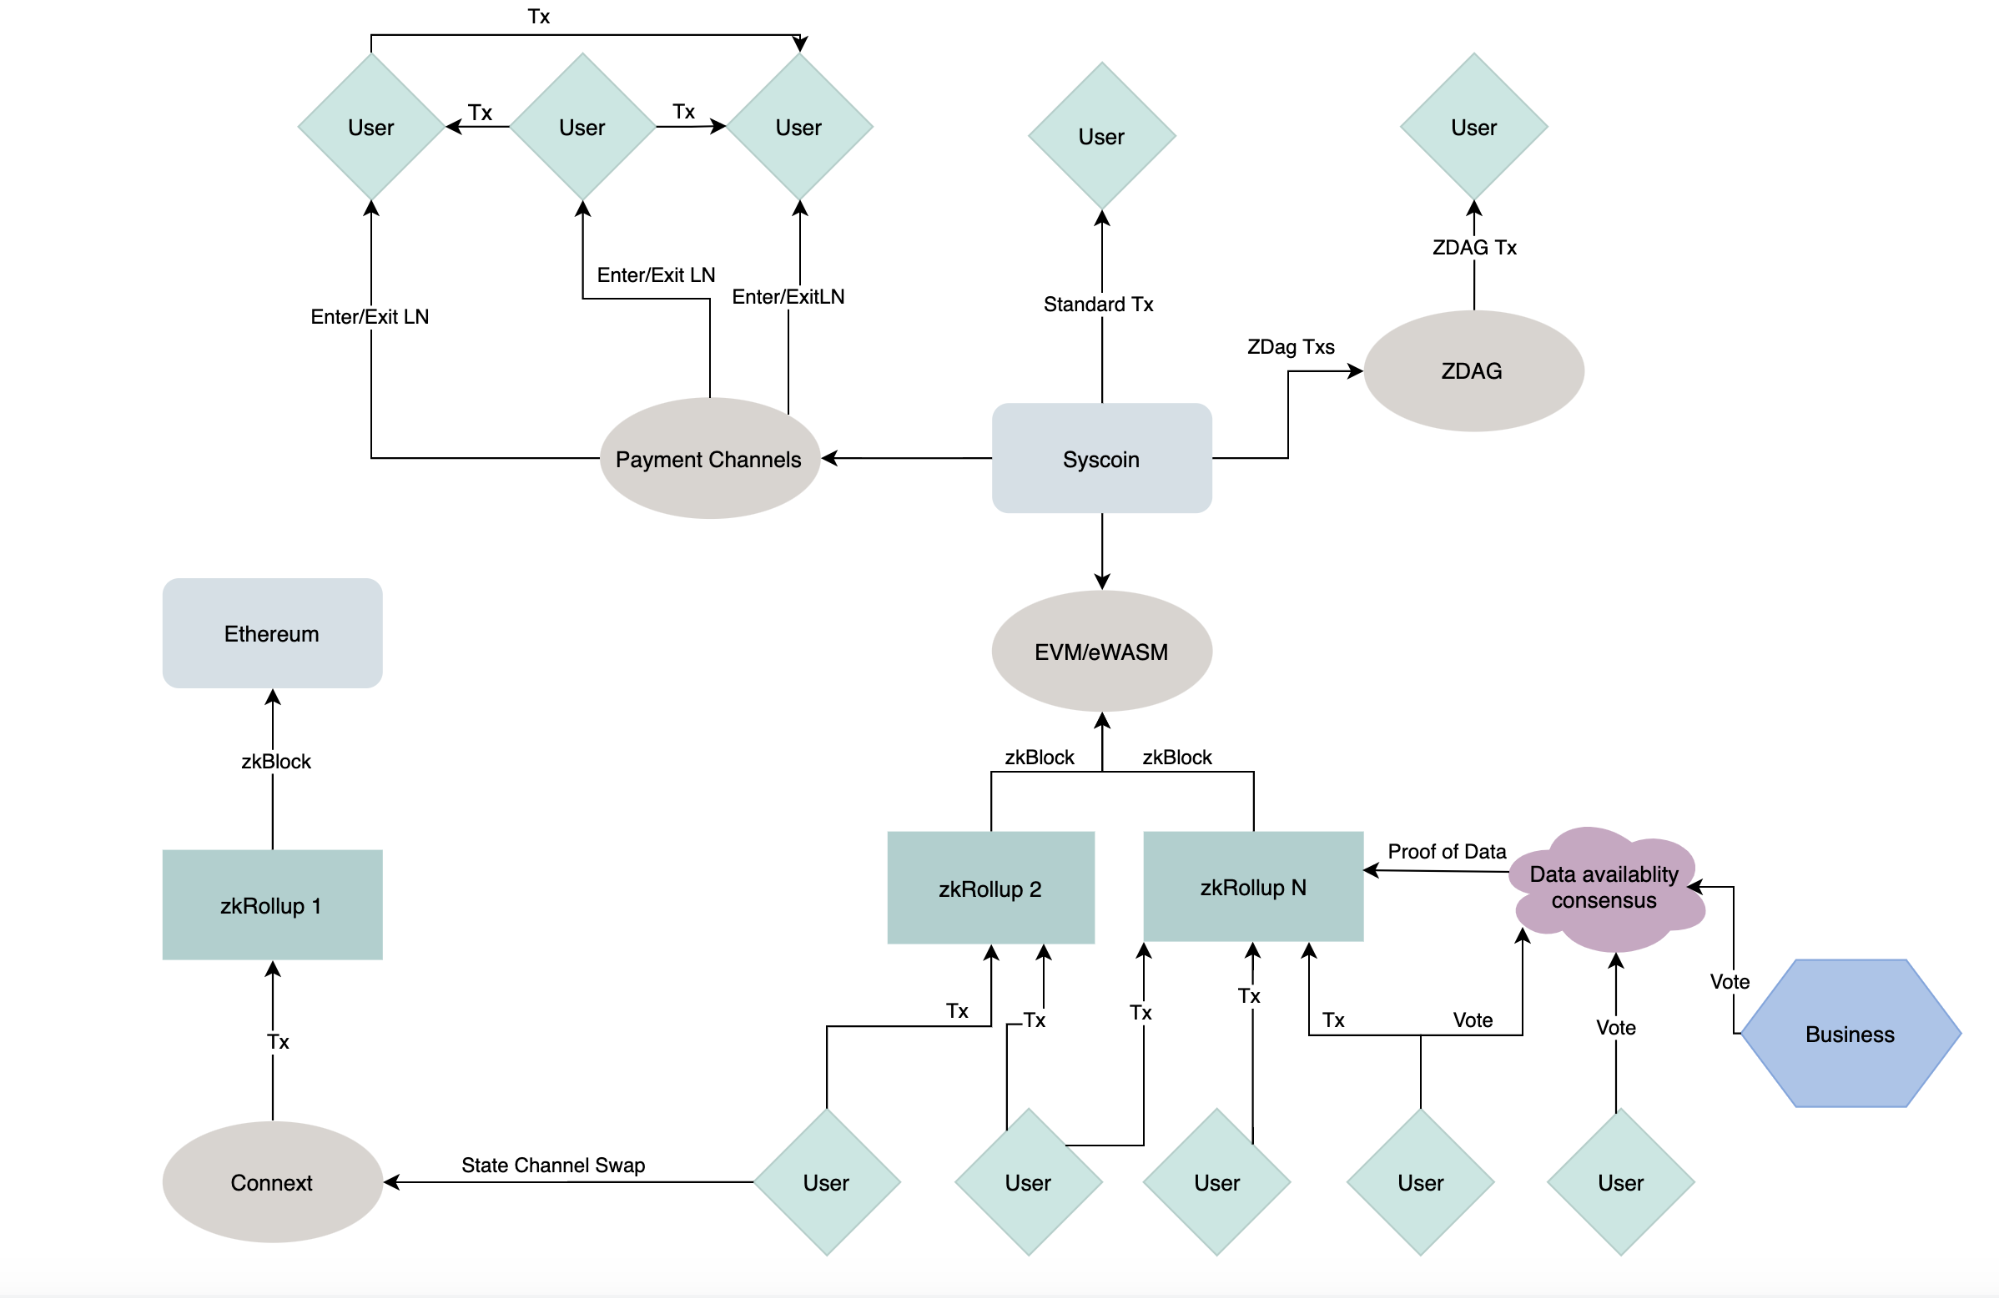
\includegraphics[width=3.4in]{img/nevm.png}
\label{fig:nevm}
\caption{Network EVM: High level description 网络EVM:高层级描述} 
\end{figure} 

\subsubsection{Optimistic vs ZkRollup}

ZKP are excellent for complex calculations above and beyond simple balance transfers. For payments, we feel UTXO payment channels combined with something like Z-DAG is an optimal solution. However, we are left with rollup solutions for generalized computation involving more complex calculations requiring consensus. ZKP非常适合用于上述复杂计算以及简单余额转移。关于支付,我们认为UTXO支付渠道与类似Z-DAG的技术相结合是最佳解决方案。但是,对于涉及需要达成共识的更复杂的一般计算,我们只有使用rollup解决方案。

The solution we adopt has to be secured by L1 consensus that is considered decentralized and secure, which Syscoin has achieved via merged-mining with Bitcoin. 我们所采用的解决方案必须由安全的、去中心化的的L1共识保护,Syscoin已通过与比特币联合挖矿实现了这一点。

There are two types of rollup solutions today: (a) Optimistic rollups (OR); and (b) zkRollups; which offer trade-offs. 目前有两种rollup解决方案:(a) Optimistic Roolup (OR);(b) zkRollups;两种方案均提供权衡。两种方案均有好有坏

Consensus about which chain or network you are working on is a difficult problem that is solved for us by Nakamoto consensus. We build on that secure longest chain rule (supplemented by Chain Locks to prevent selfish mining) to give us the world-view of the rollup states. The executions themselves can be done once by a market of provers, never to be re-executed, only verified, suggesting it becomes an almost constant cost on an arbitrarily large number of executions batched together. Given these features, OR have the same capabilities with the exception of being editable without verifying executions. The role of determining the validity of that world-view is delegated to someone watching who provides guarantees through crypto-economics. ZKPs obviate crypto-economics on execution guarantees by use of cryptography. 就您正在使用的哪条链或网络达成共识是一个难题,中本聪共识已为我们解决。为了得到rollup状态的世界观,我们以安全最长链规则(由链锁补充以防止自私挖矿)为基础。一旦执行本身可以由验证者市场完成一次,就只需进行验证,永远无需重新执行,这表明批量执行任意数量的成本几乎恒定。OR被赋予这些特征,也具有相同的功能:除了可编辑而无需验证执行。由观察谁通过加密经济提供担保的观察者来确定该世界观的有效性。ZKPs使用密码学避免了执行担保的加密经济。

Contrasting benefits between fraud proofs (optimistic) vs validity proofs (zk) can be found in \cite{Sta19}. The key takeaways from this article as to the superiority of validity proofs over fraud proofs include:

\begin{itemize}
\item Eliminate a nasty tail risk: theft of funds from OR via intricate yet viable attack vectors;
\item Reduce withdrawal times from 1–2 weeks to a few minutes;
\item Enable fast transaction confirmations and exits in practically unlimited volumes;
\item Introduce privacy by default.
\end{itemize}

欺诈证明(optimistic)与有效性证明(zk)之间的优势对比参见[38]。关于有效性证明优于欺诈证明,本文的主要结论包括:

\begin{itemize}
\item 消除严重的尾部风险:通过复杂但可行的攻击向量,盗窃OR资金;
\item 将取款时间从1-2周减到几分钟;
\item 实现快速交易确认和几乎无限量的退出;
\item 默认引入隐私。
\end{itemize}

An area often overlooked is interoperability. A generalized form of cross-chain bridging can be seen in Chain A locking tokens based on a preimage commitment by Chain B to create a zero-knowledge proof, followed by verification of that proof as the basis for manifesting equivalence on Chain B. Any blockchain with the functionality to verify these proofs could participate in the ecosystem. 区块链互操作性是一个常常被忽视的领域。跨链桥的一种广义形式可以在A链锁定代币中看到,它基于B链的原像承诺提交以创建零知识证明,然后对该证明进行验证,作为在链B上证明等效性的基础。任何具有验证这些证明功能的区块链都可以参与到这个生态系统中。

In this article we take a zkRollup-centric world-view. However, we acknowledge that it can be replaced with other technologies should they be able to serve the same purpose. As an infrastructure we are not enforcing one or the other; as developers can build on what they feel best suits their needs. We believe we are close to achieving this, and that the technology is nearing the point of being ready for the vision set forth in this article. 本文中我们采用以zkRollup为中心的世界观。但是,我们认为,如果其他技术服务目标相同,也可以将其替换。我们不会强制执行其中任何一种基础设施;开发人员可以搭建在他们认为最适合他们需求的基础上。我们相信我们将很快实现这一目标,并且支持本文这一愿景的技术也即将完成。

\subsection{Evidence 证据}

Since payment channels work with UTXOs and also benefit from on-chain scaling via Z-DAG, 16MB blocks (with segwit weight) assumed, we will see somewhere around 8MB-12MB effectively per minute (per block). We foresee that is sufficient to serve seven billion people who may enter and exit the payment channel networks once a year (ie, 2 transactions on chain per person per year) for a total of 14 Billion transactions. Let’s conservatively assume 8MB blocks and 300 bytes per transaction. Once on a payment channel, the number of transactions is not limited to on-chain bandwidth but to network related latencies and bandwidth costs. Therefore, we will conclude that our payment scalability will be able to serve billions of people doing 2 on-chain transactions per year, which is arguably realistic based on the way we envision payments to unfold; whether that is on a L2 or a payment channel network that will enable users to pay through instant transaction mechanisms. For on-chain, we have some metrics on Z-DAG throughput [1]; in the cases where someone needs to transact through point-of-sale using the Syscoin chain. The solution for payments ends up looking like a hybrid mechanism of on-chain (i.e., Z-DAG) and off-chain (i.e., payment channel) style payments. 由于支付渠道与UTXO一起运行,并且还受益于借助Z-DAG的链上扩容,假设 有16MB区块(带SegWit 重量),我们将看到每分钟(每个区块)大约 8MB-12MB有效。预计这足以为每年可能进出支付渠道网络的70亿人提供服务(即每人每年 2 笔链上交易),总计140亿笔交易。保守估计每个交易有8MB区块和300字节。一旦进入支付渠道,交易数量不再受限于链上的带宽,而是受限于网络相关的延迟和带宽成本。因此,基于我们设想的支付方式,我们的支付可扩展性能为数十亿人提供每年进行2次链上的交易服务是现实可行的;无论是在L2还是支付渠道网络上,用户都能够通过即时交易机制进行支付。对于链上,有人需要使用Syscoin链通过销售点进行交易的情况时,我们有一些关于Z-DAG吞吐量的度量[1]。支付解决方案最终看起来像是链上(即 Z-DAG)和链下(即支付渠道)式支付的混合机制。

Complex transactions such as smart contracts using zkRollups require a small amount of time to verify each proof. In this case, we assume that we will host data off-chain while using an off-chain consensus mechanism to ensure data availability for censorship resistance. Therefore, the only things that go on the chain are validity proofs. We will assume that we will assign 16MB blocks for the EVM chain per minute. 使用zkRollups的智能合约等复杂交易需要少量时间来验证每个证明。假如这样的话,我们假设我们将在链下托管数据,同时使用链下共识机制来确保数据可用性,从而抵抗审查。因此,链上只有有效性证明。我们将会假设每分钟为EVM链分配16MB区块。

In the Reddit bake-off estimates \cite{Sta20a}, Starkware showed that a proof size will be about 300kB for about 300k transactions batched together which will take about 60-80ms to verify and roughly 5 to 10 minutes to create such proofs. This was done using zk-STARKs, which present quantum resistance and no trusted setup.  Hence, zk-SNARKs offer smaller proofs and verification times at the expense of trusted setups and stronger cryptography assumptions (not post-quantum safe). We foresee that these numbers will improve over time as the cryptography improves, but current estimates suggest a rough theoretical capacity of around 1 Million offchain TPS. 在Reddit bake-off 估算 [39] 中,Starkware表明,对于大约30万笔大小将约为300kB的批量交易证明,需要约60-80毫秒的时间来验证,大约需要5到10分钟来创建这样的证明。这是使用zk-STARKs完成的,zk-STARKs具有量子抗性并且不需要可信任的设置。因此,zk-SNARKs提供更小的证明和验证时间,但需要可信的设置和更强的密码学假设(不是后量子可证安全)。我们预期随着密码学的改进,这些数字会随着时间的推移而改善,但目前粗略估算出理论容量约为100万个链下TPS。

\subsubsection{Gas Costs and Block Sizing 燃料费和区块大小}

Starkware was able to process 300k transactions over 8 blocks with a total cost of 94.5M gas; final throughput was 3000 TPS (see Reddit bake-off estimates \cite{Sta20b}). For the following calculations, let’s assume one batch-run to be 300k transactions. Ethereum can process $\sim$ 200kB of data per minute, with a cost limit of 50M gas per minute. Therefore, considering the Starkware benchmark test, and assuming a block interval of 13 seconds, we would achieve ~ 3000 TPS (ie,  300 k transactions per batch-run / (8 blocks per batch-run * 13 seconds per block)). Starkware能够处理超过8个区块的30万笔交易,总成本为9450万燃料;最终吞吐量为3000TPS(参见 Reddit bake-off估算[40])。对于以下计算,我们假设一个批次运行为30万笔交易。以太坊每分钟可以处理约200kB的数据,成本限制为每分钟50M 燃料。因此,考虑到Starkware基准测试,假设出块间隔为13秒,我们将实现3000 TPS(即,每批运行30万笔交易/(每批运行8个块* 每块13 秒))

It is estimated that Syscoin will be able to process $\sim$ 16MB of data per minute on the EVM layer (ie, NEVM in Fig 3), which is $\sim$ 80x gain over Ethereum; thus a cost limit of 4B gas (ie, 80*50M) per minute. Therefore, if the Starkware benchmark test was run on Syscoin, it is estimated that Syscoin could run the equivalent of 42 batch-runs per minute (i.e., 4B gas per minute / 94.5M gas per batch-run). That would result in an equivalent of 210k TPS (i.e., 42 batch-runs per minute * 300k transactions per batch-run / 60 seconds per minute). Syscoin将能够在EVM 层(即图3中的NEVM)上每分钟处理约16MB 的数据,这约是以太坊的80倍增益;因此成本限制为每分钟4B 燃料(即80*50M)。如果在Syscoin上运行Starkware基准测试,预计Syscoin每分钟可以运行相当于42批次处理(即,每分钟 4B 燃料 / 每次批处理 94.5M 燃料)。这相当于 210k TPS(即每分钟42次批处理* 每批运行300k事务/每分钟60秒)。

If we were to consider using Validum on the Syscoin EVM layer we estimate that we could achieve 800 batch-runs per minute (i.e., 4B gas per minute / 5M gas per batch-run). That would equate to an equivalent of 4M TPS (i.e., 800 batch-runs per minute * 300k transactions per batch-run / 60 seconds per minute). 如果我们考虑在Syscoin EVM层上使用Validum,我们预计可以实现每分钟800次批量运行(即,每分钟4B 燃料/每次批量运行5M 燃料)。这相当于4M TPS(即每分钟800次批处理*每批运行300k事务/每分钟60秒)。

\begin{figure}[h!]
\centering
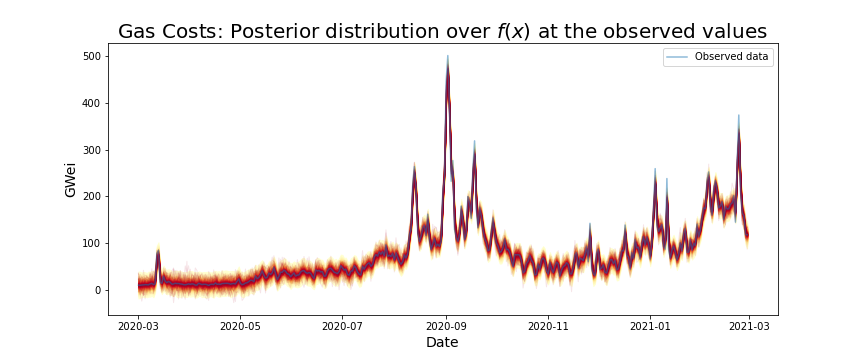
\includegraphics[width=3.7in]{img/eth_gas_costs.png}
\caption{Ethereum gas gosts in Gwei from Mar 2020 to Mar 2021. The region about the observed gas costs represents the posterior distribution of $f(x*)$ given observations, $y$, for a set of dates, $x*$; see Appendix G for details 从2020年3月至2021年3月期间以太坊的燃料费,单位为:Gwei。观察到的燃料费的区域表示给定观测值y的f(x∗) 的后验分布,x∗表示一组日期; 详见附录G。}  
\label{fig:eth_gas_costs}
\end{figure} 

\begin{figure}[h!]
\centering
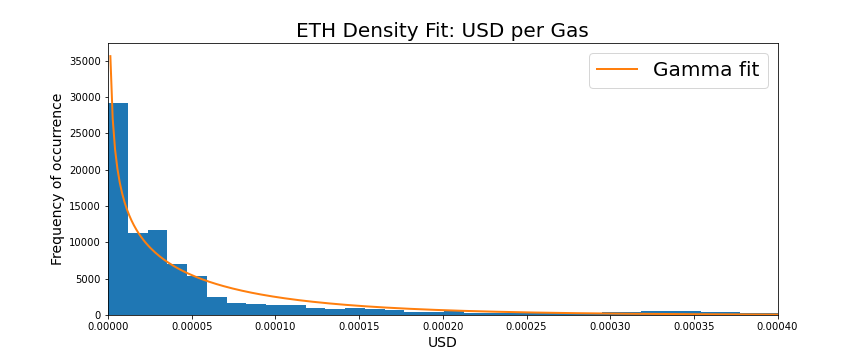
\includegraphics[width=3.7in]{img/eth_usd_density.png}
\caption{Gamma fit of Ethereum gas costs in USD using generated samples from Figure \ref{fig:eth_gas_costs} and corresponding ETHUSD prices 以太坊燃料费的Gamma fit美金价,使用图6中生成的样本和相应的ETH USD 价格} 
\label{fig:eth_usd_density}
\end{figure} 

The results from these aforementioned estimates have been tabulated in Table \ref{table:gas_cost_estimates}; more specifically, median estimates (along with its 5th and 95th percentiles) for the costs in USD terms for both ETH and NEVM. The estimates for Ethereum were determined using historical gas costs from March 2020 to March 2021 as shown in Figure \ref{fig:eth_gas_costs}, and its distribution fit in Figure \ref{fig:eth_usd_density}. 表2列出了上述估算的结果;具体而言,是ETH和NEVM以美元计算的的中位数估算值成本(连同其第5个和第95个百分位数)。以太坊的估算值是使用 2020年3月至2021年3月的历史gas成本确定的,如图6所示,其distribution fit如图7所示。

\begin{figure}[h!]
\centering
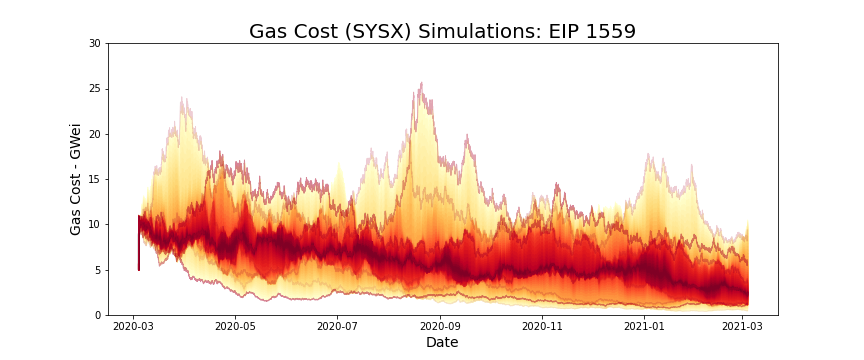
\includegraphics[width=3.7in]{img/sysx_gas_costs_eip_1559.png}
\caption{Gas cost simulations of NEVM using EIP-1559; see Appendix G. This graph shows the non-stationary decline in price over time. To our knowledge, treating this non-stationary behaviour requires better understanding of the mathematical assumptions, which have not yet been analytically researched. NEVM 的燃料费模拟使用EIP-1559;参见附录G。该图显示了价格随时间的非平稳下降。据我们所知,处理这种非平稳行为需要更好地理解尚未进行分析研究的数学假设。} 
\label{fig:sysx_gas_costs_eip_1559}
\end{figure} 

\begin{figure}[h!]
\centering
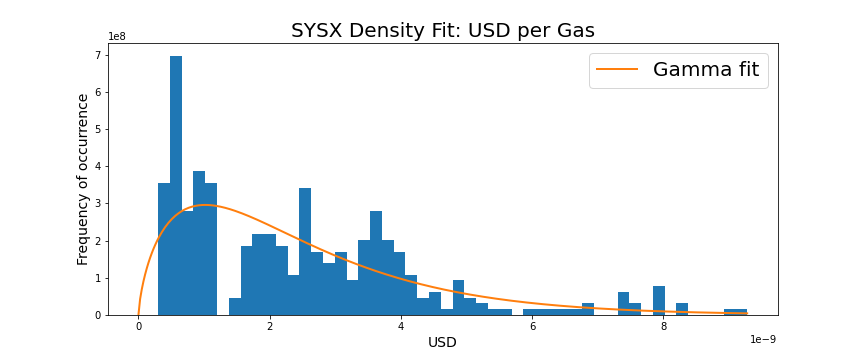
\includegraphics[width=3.7in]{img/sysx_usd_density.png}
\caption{Gamma fit of NEVM gas cost simulations in USD using generated samples from Figure \ref{fig:sysx_gas_costs_eip_1559} and SYSUSD prices from Mar 2020 to Mar 2021. These estimates are hypothetical, and will be subject to market price of SYS. Note that if significant adoption occurs due to future demand for cost effective alternatives we foresee future prices being slightly higher. NEVM 的燃料费模拟Gamma fit,使用图8中生成的样本和2020年3月至2021年3月的SYS USD价格,单位美金。这些估算是假定的,将受制于SYS 的市场价格。请注意,如果因未来对具有成本效益的替代品的需求而出现大规模使用现象,我们预计价格会略高。} 
\label{fig:sysx_usd_density}
\end{figure} 

With regards to the NEVM cost estimates, simulated gas costs were generated using Ethereum's proposed EIP-1559 (Figure \ref{fig:sysx_gas_costs_eip_1559}) and an alternative pricing mechanism that Syscoin is currently exploring. This alternative approach is called the BLock Occupancy Cost (BLOC) function (\ref{fig:bloc}), and is driven by the occupancy of the previously generated block; see Appendix D for details. 关于NEVM成本估算,模拟燃料费是使用以太坊提议的EIP-1559(图8)和 Syscoin目前正在探索的替代定价机制生成的。这种替代方法称为块占用成本(BLOC)函数(15),由先前生成的区块的占用率驱动;有关详细信息,请参阅附录D。

\begin{table*}[h!]
\centering
\begin{tabular}{ |c|c|c|c|c|c|c|   } 
\hline
Chain & Gas  Limit & Block Time & Mode & Cost  & Amortized  & Total TPS \\
 &  &  &  &  300K Tx  & Cost per Tx  &  \\ 
\hline
\multirow{3}{*}{ETH} & \multirow{3}{*}{12.5M} & \multirow{3}{*}{13 sec} & L1 & 6.3B gas  & 21,000 gas  & ~45  \\ 
\multirow{3}{*}{} & \multirow{3}{*}{} & \multirow{3}{*}{} & L2 zk-Rollup & 94.47M gas  & 315 gas & ~3,000* \\ 
\multirow{3}{*}{} & \multirow{3}{*}{} & \multirow{3}{*}{} & L2 Validium  & 5M gas  & 17 gas & ~56,000** \\ 
\hline

\multirow{3}{*}{NEVM} & \multirow{3}{*}{10B} & \multirow{3}{*}{150 sec} & L1 & 6.3B gas  & 21,000 gas  & ~3,100*\\ 
\multirow{3}{*}{} & \multirow{3}{*}{} & \multirow{3}{*}{} & L2 zk-Rollup & 94.47M gas  & 315 gas & ~210,000**\\ 
\multirow{3}{*}{} & \multirow{3}{*}{} & \multirow{3}{*}{} & L2 Validium  & 5M gas  & 17 gas & ~4,000,000 \\ 
\hline

\end{tabular}
\caption{Comparison of Gas and USD costs between ETH and NEVM. The confidence intervals for USD estimates were determined using historical gas costs for ETH (see Figure \ref{fig:eth_gas_costs}), and simulated gas costs for NEVM (see Figure \ref{fig:sysx_gas_costs_eip_1559}) using EIP-1559. ETH 与NEVM之间的Gas和USD成本比较。美元估值的置信区间是使用ETH的历史燃料费(参见图6)确定的,NEVM的模拟燃料费(参见图8)使用EIP-1559确定。}
\label{table:gas_cost_estimates}
\end{table*}

\begin{table*}[h!]
\centering
\begin{tabular}{ |c|c|c|c|c|c|c|   } 
\hline
Chain & Gas  Limit & Block Time & Mode & \multicolumn{3}{|c|}{USD / 300K Tx (Mar 20 to Mar 21) } \\
 &  300K Tx  & Cost per Tx  &  & median & lwr 5\% &  upr 95 \% \\ 
\hline
\multirow{3}{*}{ETH} & \multirow{3}{*}{12.5M} & \multirow{3}{*}{13 sec} & L1 & 159,328.24 & 10,669.40  & 1,914,394.79  \\
\multirow{3}{*}{} & \multirow{3}{*}{} & \multirow{3}{*}{} & L2 zk-Rollup & 2,389.16 & 159.99  & 28,706.81 \\ 
\multirow{3}{*}{} & \multirow{3}{*}{} & \multirow{3}{*}{} & L2 Validium  & 126.45 & 8.47  & 1,519.36 \\ 
\hline

\multirow{3}{*}{NEVM} & \multirow{3}{*}{10B} & \multirow{3}{*}{150 sec} & L1 & 1.92496 & 0.97008 & 4.51653 \\ 
\multirow{3}{*}{} & \multirow{3}{*}{} & \multirow{3}{*}{} & L2 zk-Rollup & 0.02887 & 0.01455 & 0.06773 \\ 
\multirow{3}{*}{} & \multirow{3}{*}{} & \multirow{3}{*}{} & L2 Validium  & 0.00153 & 0.00077  & 0.00358 \\ 
\hline

\end{tabular}
\caption{Comparison of Gas and USD costs between ETH and NEVM. The confidence intervals for USD estimates were determined using historical gas costs for ETH (see Figure \ref{fig:eth_gas_costs}), and simulated gas costs for NEVM (see Figure \ref{fig:sysx_gas_costs_eip_1559}) using EIP-1559. ETH 与NEVM之间的Gas和USD成本比较。美元估值的置信区间是使用ETH的历史燃料费(参见图6)确定的,NEVM的模拟燃料费(参见图8)使用EIP-1559确定。}
\label{table:gas_cost_estimates}
\end{table*}

Because of the higher throughput capabilities of baseline EVM, we may look to dynamically adjust costs of the gas limits \cite{Che17} to thwart DOS attacks. 由于基线EVM具有更高的吞吐量能力,我们可能会考虑动态调整gas limits [50] 的成本以阻止DOS攻击。

So far we have looked at EIP-1559 and the BLOC model, which both dynamically adjust gas costs. A third option we are looking at is to maintain the auctioning with a dynamic blocksize system. To facilitate this we developed a methodology driven by block failure frequency, see Appendix \ref{appendix:block_resize} for the details. 到目前为止,我们已经研究了EIP-1559和BLOC模型,它们都可以动态调整燃料费。我们正在考虑的第三个选项是使用动态区块大小系统维持拍卖。为了实现这一点,我们开发了一种由区块故障频率驱动的方法,有关详细信息,请参见附录F。

\subsubsection{Discussion 讨论}

The aforementioned calculations support the full State Safety of the main chain secured by Bitcoin, and no asynchronous network assumptions, which make theoretical calculations impractical in many other claims of blockchain throughput due to execution model bottlenecks. These results were extrapolated based on real results with constant overhead added that becomes negligible with optimizations. It is important to  note that transactions in this strategy are not re-executable; there is little to no complexity in this model other than verifying succinct proofs. The proof creation strategy is parallelized organically using this model. The verifications on the main chain can also be parallelized as they are executed on separate shards or rollup networks. Dual parallel execution and verification gives exponentially more scalability than other architectures. Additionally, depending on the business model, privacy can be built into these models at little to no extra cost. Lastly, we suggest  these are sustainable throughput calculations and not burst capacity numbers, which would be much higher (albeit with a marginally higher fee based on fee markets). For example, Ethereum is operating at 15 TPS, but there are around 150k transactions pending, and the average cost is about 200 Gwei currently. The fee rate is based on the calculation that it  takes around 10k seconds to clear, assuming this many transactions, no new transactions, and there is demand to settle earlier. Extrapolating on 4M TPS the ratio would become 40B transactions pending with 4M TPS to achieve the same fee rate on Ethereum today assuming the memory pool is big enough on nodes to support that many pending transactions. Since masternodes on Syscoin are paid to provide uptime, we can expect network bandwidth to scale up naturally to support higher throughput as demand for transaction settlement increases. Today, the ability to transact at a much higher rate using the same hardware provides greater scalability than the state-of-the-art in blockchain design without the added desired caveat of avoiding asynchronous network assumptions. We believe the proposed design will become the new state-of-the-art blockchain, which is made viable due to its security, flexibility and parallelizable computational capacity. 上述计算支持由比特币保护的主链的完整状态安全运行,并没有异步网络假设,由于模型瓶颈,这使得理论计算在许多其他区块链吞吐量要求中不切实际。这些结果是根据实际结果推断出来的,增加了恒定开销,优化后可以忽略不计。需要注意的是,该策略中的交易不可重复执行;除了验证简洁的证明外,该模型几乎无复杂性。使用该模型时,证明创建策略有机性地被并行化。因为主链上的验证在单独的分片或汇总网络上执行,它们也可以并行化。双并发执行和验证提供了比其他架构更多的指数级的可扩展性。此外,根据商业模式,隐私可以构建到这些模型中,额外成本很少甚至没有。最后,我们建议这些是可持续的吞吐量计算,而不是突发数据量,后者会高得多(尽管基于费用市场的费用略高)。例如,以太坊以15TPS运行,但有大约15万笔交易待处理,目前平均成本约为200 Gwei。费率标准是基于这样的计算:假设有很多笔交易,没有新交易并且有提前结算的需求,结算大约需要1万秒。假设节点上的内存池足够大,可以支持许多待处理的交易,那么根据4MTPS推断,该比率将变成40B交易和4M TPS待处理,以此实现与今天以太坊的相同费率。由于Syscoin上的主节点付费以提供正常运行时间,我们可以预期网络带宽会随着交易结算需求的增加而自然扩展以支持更高的吞吐量。如今,无需额外的避免异步网络假设的警告,使用相同的硬件以更高的速度进行交易的能力提供了比区块链设计中的顶尖技术更大的可扩展性。我们相信,所提议的设计由于其安全性、灵活性和可并行计算能力,将有可能成为新的顶尖区块链。

With regards to uncle rates with higher block sizes, we speculate that the NEVM will make uncle rates negligible through the use of the PoW chain mining Syscoin along with Chain Locks. We provide intuition that block sizes can be increased substantially without affecting network health. Furthermore, gas limits can be adjusted by miners up to 0.1\% from the previous block and so a natural equilibrium can form where even if more than 4B gas is required it can be established based on demand and how well the network behaves with such increases. 对于区块大小较大的叔块率,我们推测NEVM将通过使用PoW链挖掘Syscoin和链锁来使叔块率可以忽略不计。我们的直觉是,可以在不影响网络健康的情况下大幅增加区块大小。此外,矿工可以将gas limits调整为前一个区块的0.1\%,因此即使需要超过4B的燃料,也可以根据需求以及网络在这种增加时的表现情况来建立自然平衡。

\subsubsection{Decentralized Cost Model 去中心化成本模型}

Decentralized cost models lead to efficiency gains in economies of scale. We set forth a more efficient design pertaining to user intent. This design uses the UTXO model to reflect simple state transitions and a ZKP system for complex computations leading to state transitions. This leads to ideal scalability for a system by allowing people to actively make their trade-off within the same ecosystem, driven by the same miners securing that ecosystem backed by Bitcoin itself. 去中心化成本模型带来规模经济的效率收益。我们提出了与用户意图相关的更有效的设计。该设计使用UTXO模型来反映简单的状态转换,并使用ZKP系统来进行复杂的计算,从而引起状态转换。通过允许人们在同一个生态系统中积极进行权衡,由保护比特币本身支持的生态系统的相同矿工驱动,为系统带来了理想的可扩展性。

Furthermore, a decentralized cost model contributes to scalability in that ZKP gates can generalize complex computation better than fee-market resources like gas or the CPU/memory markets of EOS, etc. This leads to more deterministic and efficient consumption of resources maximizing efficiency in calculations. It also provides an opportunity for those to scale up or down based on economic incentives without creating monopolistic opportunities unlike ASIC mining. In other words, the cost is dictated by what the market can offer, via the cost of compute power (as dictated by Moore's law) instead of constrained costs of doing business on the blockchain itself. This model could let the computing market dictate the price for gas instead of being managed by miners of the blockchain. The miners would essentially only dictate the costs of the verification of these proofs when they enter the chain rather than the executions themselves. 此外,去中心化成本模型有助于可扩展性,因为ZKP gates可以更好地概括复杂的计算,优于费用市场资源,如Gas或EOS的CPU/内存市场等。这使消耗资源更确定并更加有效,使得计算效率最大化。它还为那些根据经济激励扩大或缩小规模的公司提供了机会,而不会像ASIC采矿那样创造垄断机会。换言之,成本是由市场能提供什么决定的,通过计算能力的成本(由摩尔定律决定),而不是区块链上开展业务的受限成本。这种模型可以让计算市场决定燃料价格,而不是由区块链的矿工管理。实质上在矿工进入链时只会对验证这些证明的成本进行决定,而非决定执行本身。

We can begin to see computational optimization through hardware happening with ZKP, and with a decentralized cost model it will be much simpler to understand costs of running prover services, as well as know how the costs scale based on the number of users and parameters of systems that businesses may employ. All things considered, it will be more efficient to make accurate decisions on data availability policies and the consensus systems needed to keep the system censorship resistant and secure. 我们可以开始通过 ZKP 看到通过硬件进行的计算优化,并且使用去中心化的成本模型,更易于了解运行证明者服务的成本。考虑到所有因素,在数据可用性政策和共识系统方面做出准确的决策将会更加有效,这需要保持系统审查的抵抗性和安全性。

Rollups will be friends. That is, users of one rollup system doing X TPS and users of another doing Y TPS, with the same trust model, will in effect get us to global rates of X*Y (where X is TPS of the sidechains/rollups and Y is the number of sidechains and rollups that exist). X is fairly static in that the execution models of rollups do not change drastically (and if they do, the majority of those rollup or sidechain designs end up switching to the most efficient design for execution over time). Rollups将会是很好的伙伴。也就是说,一个rollup系统的用户执行X TPS和另一个rollup系统的用户执行YTPS ,使用相同的信任模型,实际上使我们得到X*Y的全局速率(其中X是侧链/汇总的TPS,Y是存在的侧链和汇总的数量)。X是相当静态的,因为rollup 的执行模型不会发生剧烈变化(如果发生了变化,大多数这些rollup或侧链的设计最终会随着时间的推移切换到最有效的设计来执行)。

\subsection{Tokenomics 代币经济学}

A good monetary system must exhibit some form of year over year inflation in supply, which is well understood by economists. With this project, there are both inflationary and deflationary pressures pushing on the supply. Hence, it is important to ensure that the inflationary pressure coming from the block rewards outpaces the deflationary pressure coming from the fee burning. 经济学家熟知,一个好的货币系统必须表现出某种形式上年复一年的通货膨胀。在这个项目中,通货膨胀和通货紧缩的压力都在推动供应。因此,确保来自区块奖励的通货膨胀压力超过来自fee burning费用销毁的通货紧缩压力非常重要。

The current rewards for Syscoin 3 are 38.5 per block deflated 5\% per year with allocations of 67.5\% to masternodes, 22.5\% to miners and 10\% to governance proposals. When the transition to the NEVM occurs, the fee structure will change to EIP-1559 which includes: (a) an additional minting of 100M additional supply; (b) fee burning with an indeterminate block size; and (c) an elimination of max supply cap on SYS. Syscoin 3 目前的奖励是每个区块38.5,每年缩减5\%,其中67.5\%分配给主节点,22.5\% 分配给矿工,10\%分配给管理提案。当向NEVM过渡时,费用结构将更改为EIP-1559,其中包括:(a) 100M额外供应的额外铸造;(b)区块大小不确定的fee burning;(c)取消SYS的最大供应上限。

To understand the inflationary side, here is the setup under this new protocol starting Jan 2022 which is slated generate 86.8 SYS per block which occurs every 2.5 minutes. This breaks down to 58.62 SYS per block for masternodes, 19.52 SYS per block for Miners, and 8.675 SYS per block for Governance. These masternode rewards get bumped to 79.15 SYS for 1 year seniority and 117.25 SYS for 2.5 year seniority. As with Syscoin 3, the above figures will deflate 5\% per year. Once miner rewards and governance payouts reach near zero on the Syscoin mainchain, masternode holders will continue to receive SYS at a minimum of 5.275 SYS and a maximum of 10.55 SYS for full seniority nodes. An additional 0.25\% will be rewarded on the NEVM chain which will equate to 10.55 SYS per block, and will not change year over year. 为了理解通货膨胀,下面是新协议下的设置,从2022年1月开始,每块生成86.8SYS,每2.5分钟发生一次。主节点每块58.62SYS,矿工每块19.52 SYS,管理每块8.675SYS。这些主节点奖励在1年资历时达到79.15 SYS,在2.5年资历时达到117.25 SYS。与Syscoin 3一样,上述数字将每年缩减5\%。一旦 Syscoin主链上的矿工奖励和管理支出接近于零,主节点持有者将继续以最低 5.275 SYS和最高10.55SYS的全资历节点获得SYS。 NEVM链上将额外奖励 0.25\%,相当于每个区块10.55 SYS,并且不会逐年变化。

Next, to understand the deflationary side we modelled the historical transaction fee data from Ethereum as shown in Fig. \ref{fig:tx_burn}, and applied that model to our tokenomics model. For methodology, please refer to Appendix \ref{appendix:tx_fee_burn}. 接下来,为了理解通货紧缩,我们对来自以太坊的历史交易费用数据进行了建模,如图10所示,并将该模型应用于我们的代币经济学模型。方法论见附录I。

\begin{figure}[h!]
\centering
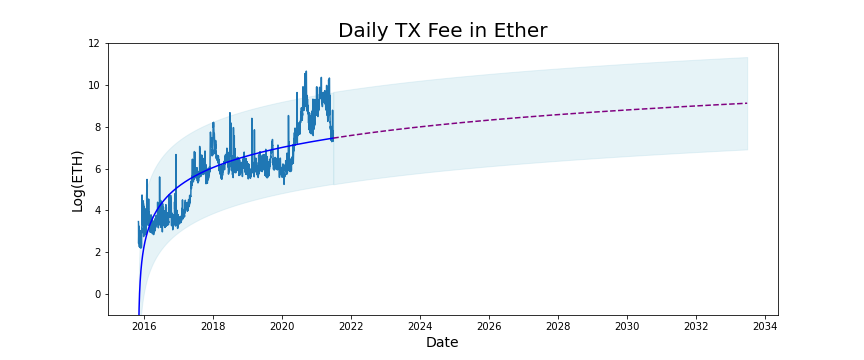
\includegraphics[width=3.7in]{img/eth_daily_tx_fee.png}
\caption{Ethereum daily transaction fee burn with projections. 以太坊每日交易fee burning,含预测值。} 
\label{fig:tx_burn}
\end{figure} 

Finally, for our supply model we combine the two components by taking the block rewards and subtracting off what is presumed to be burned through transaction fees as shown in Fig. \ref{fig:tx_delay}. For the lower bound we assume all masternodes to have less than one year seniority, and for the upper bound   we assume all masternodes to have full senority. 最后,在我们提供的模型中,我们将这两个部分组合起来,即收取区块奖励并减去交易费用,如图13所示。对于下限,我们假设所有主节点的资历都小于一年,对于上限,我们假设所有主节点都拥有完整的资历。

\begin{figure}[h!]
\centering
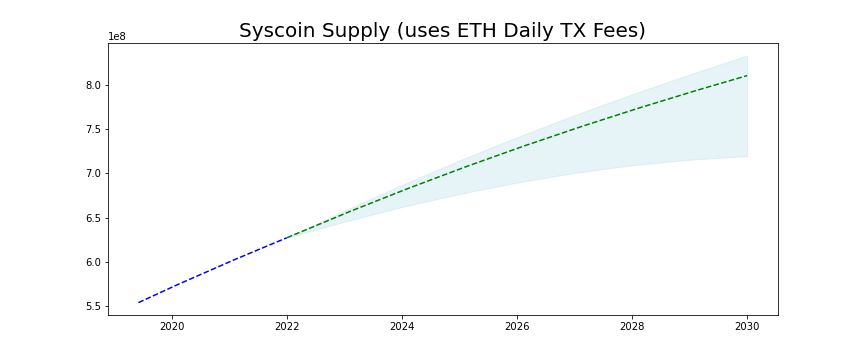
\includegraphics[width=3.7in]{img/syscoin_daily_supply.png}
\caption{Projected daily supply (Dec 6$^{th}$ start date) is comprised of two main components: (a) block rewards; and (b) fee burning. As long as the lower bound of the projected block reward growth outpaces the burn rate shown in Fig. \ref{fig:tx_burn} then supply is inflationary. 预计每日供应量(12月6日为开始日期)由两个主要部分组成:(a)区块奖励;(b) fee burning。只要预计区块奖励增长的下限超过图10中所示的消耗率,那么供应就是通货膨胀。} 
\label{fig:tx_delay}
\end{figure} 


\begin{table}[h!]
\centering
\begin{tabular}{ |c|c|c|c| } 
\hline
 & \multicolumn{3}{|c|}{ Supply } \\
 Date (1$^{st}$ of Jan) & Pred & Lwr & Upr \\
\hline
2022 & 727,569,000 & 726,910,000 & 727,822,000 \\
2023 & 753,371,000 & 744,032,000 & 756,867,000 \\
2024 & 777,884,000 & 759,626,000 & 784,452,000 \\
2025 & 801,235,000  & 773,518,000 & 810,716,000 \\
2026 & 823,358,000  & 785,487,000 & 835,584,000 \\
2027 & 844,374,000 & 795,454,000 & 859,192,000 \\
2028 & 864,340,000 & 803,267,000 & 881,560,000 \\
2029 & 883,359,000 & 808,811,000 & 902,924,000 \\
2030 & 918,496,000 & 812,038,000 & 923,102,000 \\
2031 & 934,758,000 & 812,891,000 & 942,240,000 \\
2032 & 950,250,000 & 811,302,000 & 960,400,000 \\
\hline
\end{tabular}
\caption{Supply prediction using new NEVM protocol beginning Jan 2022 through to Jan 2032 with lower and upper thresholds 从2022年1月到2032年1月使用新NEVM协议的供应预测,具有上下阈值}
\label{table:pow_vs_pos}
\end{table}

\subsection{Applications}

Commercial enterprises may start to create proprietary prover technologies where costs will be lower than market in an attempt to create an advantage for user adoption. This design is made possible since the code for the prover is not required for the verifier to ensure that executions are correct. The proof is succinct whether or not the code to make the proof is available. 商家可能会开始创建成本低于市场的专有证明人技术,从而尝试为用户采用创造竞争优势。这种设计之所以成为可能,是因为验证者不需要证明人的代码来确保执行是正确的。无论证明代码是否可用,证明都是简洁的。

While the barrier to entry is low in this industry, we have seen the open-source model and its communities optimize hardware and software and undergo academic peer review using strategies  that outpace private funded corporations. It is plausible that this will continue to play out over the long term. However, an organic market will likely form on its own, forging its own path leading to mass adoption through capitalist forces. The point here is that the privately funded vs. open source nature of proving services does not change the mechanism of secure and scalable executions of calculations that are eventually rooted to decentralized and open ledgers secured by Bitcoin. 虽然这个行业的门槛很低,但我们已经看到开源模型,其社区优化了硬件和软件,并采用了比私人投资公司更先进的策略进行学术同行审查。从长远来看,这种情况可能依然会继续发生。但以后很可能会自行形成一个有机市场,开辟自己的道路,通过资本主义力量实现大规模运用。重点是,证明服务的私人资助与开源性质并没有改变计算的安全和可扩展执行机制,这些计算最终植根于由比特币保护的去中心化和开放式分类账。

The utmost interesting propositions are the verticals that become possible by allowing infrastructure that is parameterized to scale into those economies where they are needed most, and where trust, security and auditability of value are concerns. Smart cities, IoT, AI and digital sovereignty are large markets that intersect with blockchain as a security blanket. Although ZKPs are tremendously useful on their own, applying them to consensus systems for smart contract executions drive them to another level due to the autonomous nature of “code-is-law” and provable deterministic state of logic. We believe a large part of the future economy will depend on many of the ideas presented here. Blockchain Foundry is working with commercial and enterprise adopters of blockchain technology. Our direct interaction with clients combined with our many collective years of experience in this field are reflected in this design. 最有趣的提议是通过允许参数化的基础设施扩展到那些最需要它们的经济体中,并且关注价值的信任、安全性和可审计性,从而使垂直领域成为可能。智慧城市、物联网、人工智能和数字主权是与作为安全毯的区块链相交的大市场。虽然ZKP 本身非常有用,由于“代码即法律”的自主性和可证明的逻辑确定性状态,将它们应用于智能合约执行的共识系统,会将它们推向另一个层次。但我们相信未来经济很大一部分将源自于此处的许多想法。Blockchain Foundry正在与区块链技术的商业和企业使用者合作。我们与客户的直接互动,结合多年以来我们在该领域所汲取的经验,在该设计中得以体现。

\section{Specifications 规范}
\label{section:specs}

General specifications for Syscoin 4.3:

\begin{description}[font=$\bullet$~\normalfont\scshape\color{blue!50!black}]
\item \textbf{Block time:} 150 seconds
\item \textbf{Halving interval:} 210240 (1 year)
\item \textbf{Base Rewards:}  96.25 SYS per block deflated 5 percent every 210240 blocks
\item \textbf{NEVM Rewards:}  10.55 SYS per block (not deflated). EIP1559 model
\item \textbf{Governance Proposals:}  10 percent of Base Rewards paid out every 17520 blocks (1 month)
\item \textbf{Miner/Masternode Subsidy:}  90 percent of Base Rewards. 25 percent of this value goes to miner, 75 percent of this value goes to masternode
\item \textbf{Masternode Minimum Subsidy:} 5.275 SYS (can not go below this amount even accounting for deflation)
\item \textbf{Fees:}  50/50 split between miner and masternode
\item \textbf{Consensus:} PoW is SHA256. Merge-mined with Bitcoin
\item \textbf{Masternode collateral requirement:} 100,000 SYS
\item \textbf{Masternode seniority}: 35 percent increase after 210240 blocks (1 year), 100 percent increase after 525600 blocks (2.5 years)
\end{description}

Syscoin 4.3 的一般规范:

\begin{description}[font=$\bullet$~\normalfont\scshape\color{blue!50!black}]
\item \textbf{区块时间:} 150 秒
\item \textbf{间隔减半:} 210240(1 年)
\item \textbf{ 基本奖励:}  每块 96.25 SYS ,每210240 个区块缩减 5\%
\item \textbf{奖励:}  每个区块 10.55 SYS(未压缩)。EIP1559 模型
\item \textbf{管控提案:}  每 17520 个区块(1 个月)支付10\%的基本奖励
\item \textbf{矿工/主节点补贴:}  90\%基本奖励。该值的25\% 归矿工所有,该值的75\%归主节点
\item \textbf{主节点最低补贴:} 5.275 SYS(即使考虑通货紧缩,也不能低于这个数额)
\item \textbf{费用:}  矿工和主节点之间分配50/50
\item \textbf{共识:} PoW是 SHA256。与比特币合并开采
\item \textbf{主节点抵押要求:} 100,000 SYS
\item \textbf{主节点资历}: 210240 个区块(1 年)后增长 35\%,525600 个区块(2.5 年)后增长100\%
\end{description}


\section{Summary 总结}
\label{section:summary}
We have presented what is currently under way for Syscoin 4, which will come in the form of a four-layer tech stack to work with the Ethereum ecosystem via our NEVM. With the ever-increasing cost of gas prices, we present the data showing a 1000x+ improvement over Ethereum 2.0 in efficiency in terms of low gas cost per transaction. Syscoin will utilize the best features of the top two cryptocurrencies, namely Bitcoin and Ethereum. Hence, Syscoin will provide the security offered by Bitcoin while maintaining the programmability of Ethereum. Scalable applications will be mounted on this system via ZKPs which will introduce our proposed decentralized cost model on Ethereum gas fees. 我们已经介绍了Syscoin 4目前正在开展的工作,它将以四层堆栈式技术架构形式展现,通过我们的NEVM与以太坊生态系统协同运行。随着燃料费的不断增加,我们所展示的数据显示,就每笔交易的低燃料费而言,其效率比以太坊 2.0 提高了1000 倍以上。Syscoin将充分利用比特币和以太坊这两种首屈一指的加密货币的最佳功能。因此,Syscoin将具备比特币提供的安全性,同时保持以太坊的可编程性。可扩展的应用程序通过 ZKP 安装在此系统上,ZKPs将引入我们提议的去中心化成本模型,即以太坊燃料费。

\appendices

\section{Security: PoW vs. PoS }

Proof of Stake (PoS) systems have security threats that are not inherent in Proof of Work (PoW) systems as outlined in Table \ref{table:pow_vs_pos}, of which Bitcoin employs. Hence, PoS is less secure than PoW. In terms of security, we call the Bitcoin PoW protocol the gold standard, which is the same security mechanisim that Syscoin uses. 权益证明(PoS)系统所面临的安全威胁并非工作证明(PoW)系统所固有的(见表4所示,比特币使用了这些系统)。因此,PoS安全性不如PoW。在安全性方面,我们称比特币PoW协议为黄金标准,而Syscoin所使用的安全机制与之相同。

\begin{table}[h!]
\centering
\begin{tabular}{ |c|c|c|c| } 
\hline
 & \multicolumn{3}{|c|}{ Vulnerability } \\
 Attack type & PoW & PoS & Delegated PoS \\
\hline
Short range attack & - & + & - \\
Long range attack & - & + & + \\
Coin age accumulation attack & - & maybe & - \\
Precomputing attack & - & + & - \\
Denial of service & + & + & + \\
Sybil attack & + & + & + \\
Selfish mining & - (chainlocks) & - & - \\
\hline
\end{tabular}
\caption{Comparing PoW to PoS consensus mechanism; plus sign (+) indicates vulnerability; see \cite{Bit15}. As shown, PoW system has the least number of vulnerabilities PoW与PoS共识机制的比较;加号(+)表示漏洞; 参见[14]。如图所示,PoW系统的漏洞数量最少。}
\label{table:pow_vs_pos}
\end{table}

\section{ZDAG Fundamentals Z -DAG基础知识}

Zero-Confirmation Directed Acyclic Graph (Z-DAG) is an instant settlement protocol that solves the 'fast-transaction' problem. It functions by using a Directed Acyclic Graph (DAG) where validating nodes verify the sequential ordering of transactions that are received in their memory pools. More specifically, Syscoin approach is centred around the verification of signatures and relaying of transactions. It does this by prioritizing the relay of transactions over signature verification and recipient receives funds faster; see Figure \ref{fig:dag_tx}. See Appendix A in \cite{Sidb18} for the verification process. 零确认定向非循环图((Z-DAG))是一种能解决“快速交易”问题的即时结算协议,它通过使用有向非循环图(DAG) 来运行,其中验证节点对在其内存池接收的交易排序进行验证。具体而言,Syscoin方法的核心是验证签名和中继转发交易。它通过将交易中继优先于签名验证和接收者更快地接收资金来做到这一点;参见图12。验证过程见[3]中的附录A。

\begin{figure}[h!]
\centering
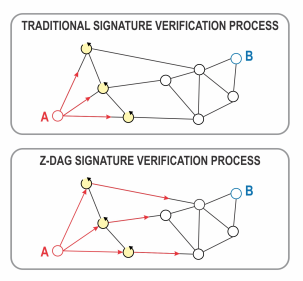
\includegraphics[width=3in]{img/dag_tx.png}
\caption{Traditional blockchain networks require each node to first check the signatures of incoming transactions before relaying them; this blocking technique bottlenecks broadcasting speed. The Z-DAG process as displayed above immediately relays transactions before checking signatures, resulting in significantly faster movement across the network. 传统区块链网络要求每个节点首先检查传入交易的签名,然后再中继它们;这种区块技术限制了广播速度。如上所示,Z-DAG过程在检查签名之前会立即中继交易,从而使整个网络中的移速明显加快。} 
\label{fig:dag_tx}
\end{figure} 


\subsection{Transmission Path 传输路径 }

The expected number of common peers between k masternodes is:
k主节点之间的普通点的预期数量是:

\begin{equation}
E\{cp_{k}\} = pk -m \left(1 - \left(1 - \frac{p}{m}\right)^{k}\right),
\end{equation}
where $p$ is the number of common peers, and $X_{i}$ is 1 when the $i^{th}$ masternode is a common peer and 0 otherwise. The probability of having $n$ common peers is given by: 
其中p是普通点的数量,当$i^{th}$主节点是一个普通点时,$X_{i}$是1,否则为0。有n个普通点的概率由下式得出:

\begin{equation}
P(|cp| = n) = \frac{\binom{M}{c} \binom{M-c}{p-c} \binom{M-p}{p-c} }{\binom{M}{p}}
\end{equation}

\subsection{Transmission Delay 传输延迟}

Using a dataset (containing 2086 samples) of average transmission times of ten transmissions between two hosts, it was modelled using the Gamma distribution as shown in Figure \ref{fig:tx_delay}. Using this model, the probability of transmission arriving in a given time can be estimated at various time points. 使用两台主机之间十次传输的平均传输时间数据集(包含2086个样本),通过伽马分布对其进行建模,如图13所示。使用该模型,可以估算出在不同的时间节点,指定时间内传输到达的概率。

\begin{figure}[h!]
\centering
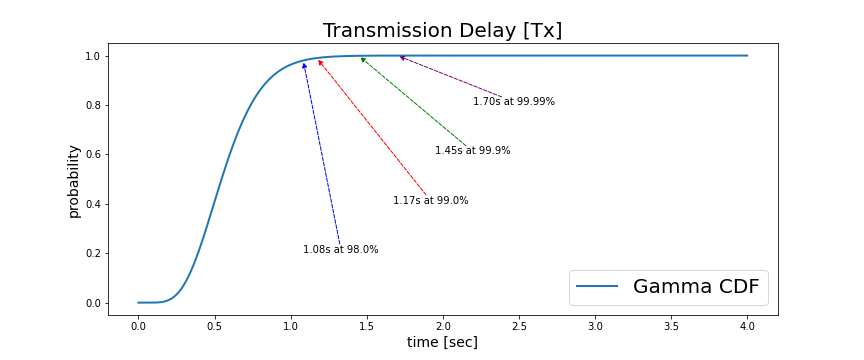
\includegraphics[width=3.7in]{img/transmission_delay.png}
\caption{Probability of Tx arrival after $5$ hops modelled via $X \sim Gamma(7.358,0.0777)$} 
\label{fig:tx_delay}
\end{figure} 

\section{Zero Knowledge Proofs Fundamentals 零知识证明基础}

The motivation of a Zero Knowledge Proof (ZKP) is to allow for one party (ie, prover) to convince another party (ie, verifier) of facts without revealing information (ie, zero knowledge). An example of a ZKP would be: allowing a subscriber (ie, prover) to gain access to an online service (ie, verifier) without revealing any personal data, other than the fact than that party is a paid subscriber. A ZKP must satisfy three conditions:
\begin{enumerate}
\item \textbf{Completeness:} If statement is true, verifier will be convinced by prover
\item\textbf{Soundness:} If statement is false, a cheating prover cannot (except with some small probability) convince verifier it is true
\item \textbf{Zero-knowledge:} If statement is true, verifier knows nothing else
\end{enumerate}

零知识证明(ZKP)是指允许一方(即证明者)在能够在不向验证者提供任何有用的信息(即零知识)的情况下,使另一方(即验证者)相信某个论断是正确的。例如:允许订阅者(即证明者)访问在线服务(即验证者),而不披露任何个人数据(除非该方是付费订阅者)。ZKP必须满足以下三个条件:
\begin{enumerate}
\item \textbf{完备性:} 如果这个陈述是真的, 验证者将被验证者说服。
\item\textbf{可靠性:} 如果陈述是假的,欺诈证明人没法(除非有很小的概率)说服验证者它是真的。
\item \textbf{零知识性:} 如果该陈述为真,则除此之外,验证者不会获悉其他任何东西。
\end{enumerate}

\begin{figure}[h!]
\centering
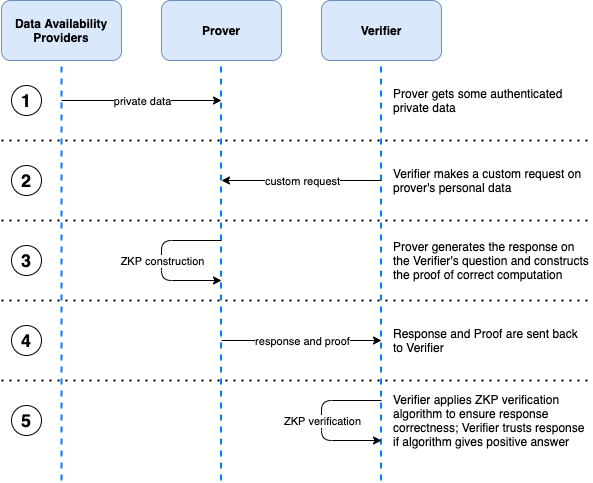
\includegraphics[width=3.7in]{img/zkp.png}
\caption{Data exchange in a Zero-knowledge proof system} 
\label{fig:zkp}
\end{figure} 

There are two types of ZKP:
\begin{enumerate}
\item \textbf{Interactive ZKP:} Comprised of multiple challenge / response messages (commitment, challenge and response); requires a stable communication channel
\item \textbf{Non-interactive ZKP:} Only needs single message and is more efficient; can be run offline
\end{enumerate}

ZKP有两种类型:
\begin{enumerate}
\item \textbf{交互式ZKP:} 由多个挑战/响应消息(承诺、挑战和响应)组成;需要一个稳定的通信通道;
\item \textbf{非交互式ZKP:} 只需要单一消息,效率更高;可脱机运行。
\end{enumerate}

zk-SNARK and zk-STARKS are types of Non-interactive ZKP , where no interaction is required between prover and verifier. zk-SNARK 和 zk-STARKS 是非交互式 ZKP 的类型,证明者和验证者之间无需交互。

\section{Block Occupancy Cost (BLOC) Function 区块占用成本 (BLOC) 函数}

We considered two approaches to model the gas costs, $y_{c,k}$ at the $k^{th}$ block, using model 1:
我们考虑用两种方法给燃料费建模,$y_{c,k}$ 在 $k^{th}$ 区块上,使用模型1:

\begin{equation}
\mathbf{y}_{c,k} = \dfrac{1}{\gamma}\log\left(\dfrac{1+\mathbf{x}_{o,k-1}}{1-\mathbf{x}_{o,k-1}}\right) + \mathbf{y}_{c,0};
\end{equation}
and model 2:
\begin{equation}
\mathbf{y}_{c,k} = \left| \dfrac{1}{\gamma(\mathbf{x}_{o,k-1}-1)} \right| + y_{c,0} - \dfrac{1}{\gamma},
\end{equation}
where $x_{o,k} \in [0,1] \forall k$ is the block occupancy, $y_{c,0}$ is the base cost, and $\gamma$ is an adjustable scaling term. We call $y_{c}$ the BLock Occupancy Cost (BLOC) function; see Figure \ref{fig:bloc}. 其中 $x_{o,k} \in [0,1] \forall k$ 是区块占用率,$y_{c}$ 是基本成本,γ 是一个可扩展项。 我们称yc为区块占用成本(BLOC) 函数;见图15。

\begin{figure}[h!]
\centering
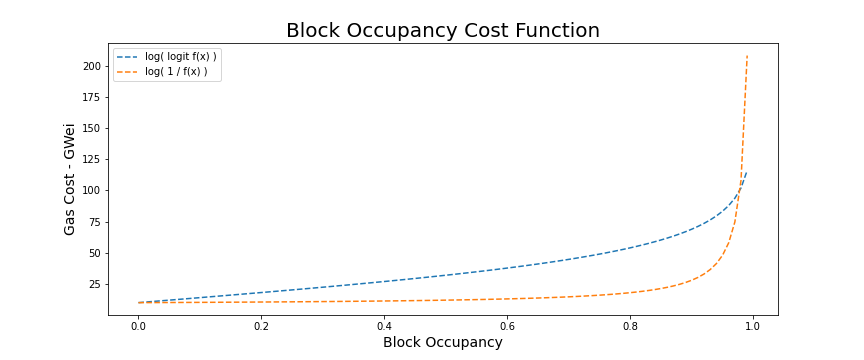
\includegraphics[width=3in]{img/blk_occupancy_cost_fn.png}
\caption{BLock Occupancy Cost (BLOC) functions; model 1 and 2 可以使用yc的其他变体来突显各种特性。例如,模型1具有波动较小的特点,但预期基本成本高于模型2。} 
\label{fig:bloc}
\end{figure} 

Other variants of \textbf{y}$_{c}$ can be utilized highlighting various characteristics. For instance, Model 1 has the characteristic of being less volatile, but with a higher expected base cost than Model 2. 可以使用yc的其他变体来突显各种特性。例如,模型1具有波动较小的特点,但预期基本成本高于模型2。

\section{Block Occupancy and Gas Simulations 区块占用和Gas模拟}

To simulate arbitrary block occupancies, we use the Beta distribution:
为了模拟任意区块占用,我们使用了Beta分布:

 \begin{equation}
\mathbf{x}_{o,t} \sim Beta(\alpha_{t},\beta_{t})
 \end{equation}
 where $t$ is time, and $\beta_{t} = 1-\alpha_{t}$. 其中t是时间,$\beta_{t} = 1-\alpha_{t}$.
 
To exhibit slow upward growth over time for $\alpha_{t}$, we used a MinMax scaled ARIMA(0,1,1) model, otherwise known as a simple exponential smoothing model with growth, which is of the form:
为了展示αt随着时间缓慢向上增长,我们使用了MinMax缩放ARIMA(0,1,1)模型,也称为一同增长的简单指数平滑模型,公式为:

\begin{equation}
\hat{\alpha'}_{t} = \mu + \alpha'_{t-1} - \theta_{1}\epsilon_{t},
\end{equation}
and then applied MinMax scaling to ensure $\alpha_{t} \in [0,1]$:
然后应用MinMax缩放以确保 $\alpha_{t} \in [0,1]$:
\begin{equation}
\hat{\alpha_{t}} = \dfrac{\alpha'_{t} - min(\alpha'_{t})}{  max(\alpha'_{t}) - min(\alpha'_{t}) }.
\end{equation}

Block Occupancy simulations, \textbf{x}$_{o,t}$, were fed into the BLOC function, to achieve a set of gas simulations, \textbf{y}$_{c,t}$, at each instance of time $t$. 区块占用模拟,\textbf{x}$_{o,t}$被输入到BLOC函数中,以在时间t的每个实例中实现一组gas模拟\textbf{y}$_{c,t}$。

\section{Block Resize on Failure Model 故障模型的区块调整}
\label{appendix:block_resize}

This Block Resize on Failure model dynamically adjusts the blocksize based on time to last block failure. If the time interval between failures is short then the probability of failure is high and the size for the next block gets decreased. However, when the time interval between failures is long then the probability of failure is low and the size for the next block size gets increased. This methodology is updated upon each failure, and consists of three main steps which include:

\begin{itemize}
\item Generate a Kaplan Meier estimator based on last N failures
\item Using time interval between last failure get estimated probability of failure using Kaplan Meier estimator
\item Feed the estimated probability of failure into a block size transfer function to get the block size adjustment for the next block
\end{itemize}

此故障模型的区块调整根据上次区块故障的时间动态调整区块大小。如果故障之间的时间间隔很短,则发生故障的概率很高,并且下一个区块的大小会减小。而当故障之间的时间间隔很长时,则出现故障的概率很低,并且下一个区块大小的大小会增加。此方法论将在每次故障时更新,由三个主要步骤组成,其中包括:

\begin{itemize}
\item 依据最近的N故障生成Kaplan Meier估计量;
\item 使用上次故障之间的时间间隔,通过使用Kaplan Meier估计量估算故障概率;
\item 将估计的失败概率输入区块大小传递函数以获得下一个区块的区块大小调整信。
\end{itemize}

The goal of the Kaplan Meier estimator is to estimate the survival function, $S$, defined as:
Kaplan Meier估计量的目标是评估生存函数S,定义为:
\begin{equation}
S(t) = Pr(\tau > t),
\end{equation}
where $t$ is time, and  $\tau > 0$ be a random variable. The survivor function for the Kaplan Meier estimator function is given by:
其中$t$是时间, $\tau > 0$ 是一个随机变量。Kaplan Meier估计量函数的生存函数由下式给出:
\begin{equation}
\hat{S}(t) = \prod_{i; t_{i} < t} 1- \frac{d_{i}}{n_{i}}
\end{equation}
where $t_{i}$ is a time when at least one black failure happened, $d_{i}$ the number of failures, and $n_{i}$ the blocks that have not failed. 其中ti是至少发生一次黑屏故障的具体时间,$d_{i}$是故障的次数,$n_{i}$是无故障区块。 

The block size transfer function constructed from the following logit function:
由以下logit函数构造的区块大小传递函数:
\begin{equation}
y_{tr} = -2*A*\frac{e^{k(x-x_{0})}}{1+e^{k(x-x_{0})}} + A
\end{equation}
where preconfigured parameters ${A,k}$  determine how aggressive the resizing is upon each block failure. These parameters are typically determined aprior based on simulations run on the test net. 其中预先配置的参数A、k决定每个区块故障时调整大小的积极程度。这些参数通常是基于在测试网上运行的模拟预先确定的。

\section{EIP-1559}

EIP-1559 is a new proposed pricing mechanism for the Ethereum protocol that includes a stationary network fee during states of no congestion which dynamically adjusts during states of congestion. The original gas fee model uses a auction system where miners choose transactions with the highest bids. This has led to several inefficiencies such as instability of blockchains with no reward, needless delays, fee overpayment, and mismatch fee levels between volatility ad social cost. EIP-1559 是一种新提出的以太坊协议定价机制,包括在无阻塞状态下的固定网络费用,在阻塞状态下动态调整。原始的燃料费模型使用拍卖系统,矿工选择出价最高的交易。这导致效率低下,例如没有奖励的区块链不稳定、不必要的延迟、费用多付以及波动性和社会成本之间的费用水平不匹配。

The basic premise of the new proposal begins with setting the base fee which increases when the network capacity exceeds the target per-block gas usage, and decreases when the capacity is below the target. The calculation of the updated basefee, $b_{k+1}$ at the $k+1^{th}$ block,  is as follows:
新提案的基本前提是设置base fee,当网络容量超过目标每块燃料使用量时增加,当容量低于目标时减少。更新后的basefee,$b_{k+1}$ 在第$k+1^{th}$个区块的计算如下:

\begin{eqnarray} \label{eq:eip1559}
b_{k+1} = b_{k} f_{k}, \\
f_{k} = 1 + \dfrac{\delta_{k}}{c}
\end{eqnarray}
where $\delta_{k} = usage_{k} - target~gas~fee$, and $c = (target)*(basefee~max~change)$. 其中$\delta_{k}$ = 使用量 k − 目标gas fee,c = (target) ∗ (basefee max change)。

Ideally, we would like to see $b_{k}$ behave as a stationary process for states of congestion and non-congestion. A stationary process is when $b_{k}$ and $b_{k+N}$ have the same probability distributions for all N. Hence, this research problem can be broken into these two main categories. We foresee the latter problem being significantly more difficult to mathematically model than the former, as there are many non-stationary edge-cases that can arise from various attacks which have not yet been defined. For the sake of brevity, we assume $\delta_{k}$ to be a stationary Gaussian process in this discussion. 理想情况下,我们希望看到bk表现为阻塞和非阻塞状态的平稳过程。平稳过程是当bk和bk+N对所有N具有相同的概率分布时。因此,这个研究问题可以分为这两个主要类别。我们预见到后一个问题比前一个问题更难以运用数学建模,因为有许多非平稳的边缘情况可能来自尚未定义的各种攻击。为简洁起见,在本次讨论中,我们假设 δk 是一个平稳的高斯过程。

It is quite possible that this problem can be addressed using a state space model or some other kind of probabilistic graphical model. Approaching the problem this way could be an effective way of optimally ensuring (under predefined assumptions) that the statistics of $\delta_{k}$ stay relatively stable over $k$, and a good way to mathematically define various attack vectors. 这个问题很可能可以使用状态空间模型或其他某种概率图形模型来解决。 以这种方式解决问题将会是优化确保(在预定义的假设下)δk 的统计数据在 k 上保持相对稳定的一种有效方法,也是一种在数学上定义各种攻击向量的好方法。

\section{Gaussian Processes 高斯过程}
\label{appendix:marginal}

Assume observed data, $y$, are the sum of a Gaussian Process (GP) and Gaussian noise, given by:
假设观察到的数据 $y$ 是高斯过程 (GP) 和高斯噪声的总和,由下式给出:

\begin{eqnarray}
\mathbf{y} = f(x) + \mathbf{\epsilon}  \\
\mathbf{\epsilon}  \sim N(0,\Sigma) 
\end{eqnarray}
The unknown function, $f(x)$, is modelled as:
未知函数  $f(x)$ 被建模为:

\begin{equation}
f(x) \sim GP(\mu(x), k(x,x')),
\end{equation}
where $\mu(x)$ and $k(x,x')$ are the mean and covariance function respectively; the covariance function is often called the kernel function, and can take on several forms based on the structure of the input data, $x$. In this work, we use the Matern 5/2 kernel, which is of the form:
其中 $\mu(x)$ 和 $k(x,x')$ 分别是均值和协方差函数;协方差函数通常称为核函数,可以根据输入数据 $x$ 的结构采用多种形式。此项中,我们使用 Matern 5/2 kernel,公式为:

\begin{equation}
k(x,x') = \left( 1 + \dfrac{\sqrt{g(x,x')}}{\ell} + \dfrac{g(x,x')}{3\ell^2}\right)\exp\left[ \dfrac{g(x,x')}{\ell} \right]\ 
\end{equation}
where 其中:
\begin{equation}
	g(x,x') = 5(x-x')^2.
\end{equation}

For this work, we looked at observations, \textbf{y}, probabilistically, which can be determined via:
此项中,我们用概率统计观察了观测值 y,它可以通过以下方式确定:
\begin{equation}
p(y|x) = \int p(y | f,x) p (f, |x) df;
\end{equation}
this is otherwise known as the marginal likelihood; from a Bayesian context, this may be referred to as the evidence, which is the normalizing part of Bayes rule. The marginal likelihood can be utilized to generate conditional distribution for Gaussians to get the posterior distribution of $f(x*)$ given \textbf{y}. To do this we used Markov Chain Monte Carlo (MCMC) sampling using the PyMC3 python package; for more detail along with coding examples, see \cite{Fon20}. 这也称为边际可能性;从贝叶斯上下文来看,这可以称为证据,这是贝叶斯规则的规范化部分。边际可能性可用于生成高斯分布的条件分布,从而获取给定 y 的 f(x∗) 的后验分布。为此,我们使用 PyMC3 python包使用Markov Chain Monte Carlo (MCMC) 采样,有关编码示例的更多详细信息,请参见 [51]。

\section{Tokenomics: Transaction Fee Burn 代币经济学:交易费燃烧}
\label{appendix:tx_fee_burn}

To model transaction fee burn to determine the supply end we used Ethereum fee data to serve as a proxy. We have determined that transaction fees follow an exponential growth that can be modelled via the following log-log model:
为了模拟交易费燃烧从而确定供应端,我们使用以太坊费用数据作为代理。我们已经确定交易费用遵循指数增长,可以通过以下 log-log 模型建模:
\begin{equation}
ln(y) = a + bln(x)
\end{equation}
where parameters $a$ and $b$ and its confidence intervals can be estimated using Ordinary Least Squares (OLS). 其中参数a和b及其置信区间可以使用普通最小二乘法(OLS)进行估算。

\begin{thebibliography}{00}

\bibitem{Sig21} J. Sidhu, \textit{A Design For An Efficient Coordinated Financial Computing Platform}, Feb 2021, Accessed on: Sep 2021.  [Online]. Available:  https://jsidhu.medium.com/a-design-for-an-efficient-coordinated-financial-computing-platform-ab27e8a825a0

\bibitem{Sida18} J. Sidhu, \textit{Syscoin 3.0: A Peer-to-Peer Electronic Cash System Built For Business Applications}, Blockchain Foundry Inc, Feb. 2018. Accessed on: Dec 2020. [Online]. Available: https://syscoin.org/$syscoin3_whitepaper.pdf$

\bibitem{Sidb18} J. Sidhu, E, Scott, and A. Gabriel, \textit{Z-DAG: An interactive DAG protocol for real-time crypto payments with Nakamoto consensus security parameters}, Blockchain Foundry Inc, Feb. 2018. Accessed on: Dec 2020. [Online]. Available: https://syscoin.org/$syscoin3_whitepaper.pdf$

\bibitem{But19} V. Buterin,  \textit{Blockchain Resource Pricing}, Apr 2019. Accessed on: May 2021. [Online]. Available: https://github.com/ethereum/research/blob/master/papers/pricing/ethpricing.pdf

\bibitem{Som15} Y. Sompolinsky, and A. Zohar, \textit{Secure High-rate Transaction Processing in Bitcoin}, Proc. 19th Int. Conf. Financial Cryptogr, Data Secur. (FC’20), Jan 2015, pp. 507-527

\bibitem{Som18} Y. Sompolinsky, and A. Zohar, \textit{PHANTOM: A Scalable BlockDAG Protocol}, IACR Cryptol. ePrint Arch., vol 2018, 2018,  pp. 104

\bibitem{Bir20} G. Birmpas, E. Koutsoupias, P. Lazos, F.J. Marmolejo-Cossío, \textit{Fairness and Efficiency in DAG-Based Cryptocurrencies}, Proc. 24th Int. Conf. Financial Cryptogr, Data Secur. (FC’15), Jan 2015, pp. 507-527

\bibitem{Bre12} Eric Brewer, \textit{CAP twelve years later: How the 'rules' have changed}, Computer, Volume 45, Issue 2 (2012), pg. 23–29

\bibitem{Nor19} N. Word, \textit{UTXO vs Global State}, Nov. 2019. Accessed on: Jan 2021. [Online]. Available: https://word.site/2019/11/20/utxo-vs-global-state/

\bibitem{Szt15} P. Sztorc \textit{Nothing is Cheaper than Proof of Work}, Aug. 2015. Accessed on: Jan 2021. [Online]. Available: https://www.truthcoin.info/blog/pow-cheapest/

\bibitem{Eya18} I. Eyal, and E.G. Sirer, \textit{Majority is not Enough: Bitcoin Mining is Vulnerable}, \emph{Communications of the ACM}., vol. 61, no. 7, Jun. 2018.

\bibitem{Cao20} B. Cao, Z. Zhang, D. Feng, S. Zhang, L. Zhang, M. Peng, and
Y Li, \textit{Performance analysis and comparison of PoW, PoS and DAG based blockchains}, \emph{Digital Communications and Networks}., vol. 6, no. 4, Nov. 2020, pp 480-485

\bibitem{But20} V. Buterin, \textit{Using polynomial commitments to replace state roots}, Ethereum Research, Mar. 2020. Accessed on: Jan 2021. [Online]. Available: https://ethresear.ch/t/using-polynomial-commitments-to-replace-state-roots/7095

\bibitem{Bit15} G., \textit{Proof of Stake Versus Proof of Work. Technical Report}, BitFury Group, 2015. Accessed on: Jan 2021. [Online]. Available: http://bitfury.com/content/5-white-papers-research/pos-vs-pow-1.0.2.pdf 

\bibitem{Duf18} E. Duffield, and D. Diaz, \textit{Dash: A Payments-Focused Cryptocurrency}, Dash, Aug 2018. Accessed on: Jan 2021. [Online]. Available: https://github.com/dashpay/dash/wiki/Whitepaper

\bibitem{BitCore} \textit{Bitcoin Core FAQ, Compact Blocks FAQ}, Accessed on: Feb 2021. [Online]. Available: https://bitcoincore.org/en/2016/06/07/compact-blocks-faq/

\bibitem{Blo18} ] A. Block, \textit{Mitigating 51\% attacks with LLMQ-based ChainLocks}. Accessed on: Feb 2021. [Online], Nov 2018. Available: https://blog.dash.org/mitigating-51-attacks-with-llmq-based-chainlocks-7266aa648ec9

\bibitem{Val19} J. Valenzuela, Andreas Antonopoulos, \textit{Calls Dash Chain Locks “a Smart Way of” Preventing 51\% Attacks}. Aug 22, 2019. Accessed on: Feb 2021. [Online]. Available: https://dashnews.org/andreas-antonopoulos-calls-dash-chainlocks-a-smart-way-of-preventing-51-attacks/

\bibitem{Bon18} D. Boneh, M. Drijvers, and G. Neven, \textit{BLS Multi-Signatures With Public-Key Aggregation}, Mar 2018. Accessed on: Feb 2021. [Online]. Available: https://crypto.stanford.edu/~dabo/pubs/papers/BLSmultisig.html

\bibitem{Dra18} J. Drake. \textit{Pragmatic signature aggregation with BLS}, May 2018. Accessed on: Feb 2021. [Online]. Available:  https://ethresear.ch/t/pragmatic-signature-aggregation-with-bls/2105

\bibitem{Bow17} S. Bowe, \textit{BLS12-381: New zk-SNARK Elliptic Curve Construction}, Mar 2017. Accessed on: Feb 2021. [Online]. Available: https://electriccoin.co/blog/new-snark-curve/

\bibitem{Blo18}  A. Block, \textit{BLS: Is it really that slow?}, Jul 2018. Accessed on: Feb 2021. [Online]. Available: https://blog.dash.org/bls-is-it-really-that-slow-4ca8c1fcd38e

\bibitem{Rou17}  S. de la Rouvier. \textit{Interplanetary Linked Computing: Separating Merkle Computing from Blockchain Computational Courts}, Jan 2017. Accessed on: Feb 2021. [Online]. Available: https://media.consensys.net/interplanetary-linked-computing-separating-merkle-computing-from-blockchain-computational-courts-1ade201ecf8a

\bibitem{Ano18} Anonymous Kid, Why the fuck did Satoshi implement the 1 MB blocksize limit? [Online forum comment], Jan 2018, Accessed on: Feb 2021. [Online]. Available:  https://bitcointalk.org/index.php?topic=2786690.0

\bibitem{Zer21} \textit{Zero-Knowledge Proofs What are they, how do they work, and are they fast yet?} Accessed on: Feb 2021. [Online]. Available: https://zkp.science/

\bibitem{Ben18} E. Ben-Sasson, I. Bentov, Y. Horesh, and M. Riabzev, \textit{Scalable, transparent, and post-quantum secure computational integrity}, IACR Cryptol, 2018, pp 46 

\bibitem{Dry19} Dryja, T, Utreexo: A dynamic hash-based accumulator optimized for the bitcoin UTXO set, IACR Cryptol. ePrint Arch., 2019, p. 611.

\bibitem{Hot19} G.I. Hotchkiss, \textit{The 1.x Files: The State of Stateless Ethereum}, Dec 2019. Accessed on: Feb 2021. [Online]. Available:   https://blog.ethereum.org/2019/12/30/eth1x-files-state-of-stateless-ethereum/

\bibitem{Bow18} S. Bowe, A. Chiesa, M. Green, I. Miers, P. Mishra, H. Wu: \textit{Zexe: Enabling decentralized private computation}. Cryptology ePrint Archive, Report 2018/962 (2018). Accessed on: Feb 2021. [Online]. Available:  https://par.nsf.gov/servlets/purl/10175111

\bibitem{Nil20} A. Nilsson, P.N. Bideh, J. Brorsson, \textit{A survey of published attacks on Intel SGX}. 2020, arXiv:2006.13598

\bibitem{Nel18} C. Nelson, \textit{Zero-Knowledge Proofs: Privacy-Preserving Digital Identity}, Oct 2018. Feb 2021. Accessed on: [Online]. Available: https://www.slideshare.net/SSIMeetup/zeroknowledge-proofs-privacypreserving-digital-identity-with-clare-nelson

\bibitem{Bon19} D. Boneh, \textit{Discrete Log based Zero-Knowledge Proofs}, Apr 2019,  Accessed on: Feb 2021 [Online].  Available: https://www.youtube.com/watch?v=wB3DlND7KEw

\bibitem{Qua18} \textit{Quantum Computing’s Implications for Cryptography (Chapter 4)}, National Academies of Sciences, Engineering, and Medicine: Quantum Computing: Progress and Prospects. The National Academies Press, Washington, DC, 2018.

\bibitem{Nai19} S. Naihin, \textit{Goodbye Bitcoin… Hello Quantum}, Apr 2019, Accessed on: Feb 2021 [Online].   https://www.linkedin.com/pulse/goodbye-bitcoin-helloquantum-silen-naihin

\bibitem{Nas19} L.T. do Nascimento, S. Kumari, and V. Ganesan, \textit{Zero Knowledge Proofs Applied to Auctions}, May 2019, Accessed on: Feb 2021 [Online].   Available: https://courses.csail.mit.edu/6.857/2019/project/18-doNascimento-Kumari-Ganesan.pdf

\bibitem{But17} V. Buterin and V. Griffith, Casper the Friendly Finality Gadget. CoRR, Vol. abs/1710.09437, 2017. arxiv: 1710.09437, http://arxiv.org/abs/1710.09437

\bibitem{Neu21} M. Neuder, D.J. Moroz, R. Rao, and D.C. Parkes, \textit{Low-cost attacks on Ethereum 2.0 by sub-1/3 stakeholders}, 2021. arXiv:2102.02247,  https://arxiv.org/abs/2102.02247

\bibitem{Sta19} Starkware, \textit{Validity Proofs vs. Fraud Proofs}, Jan 2019, Accessed on: Feb 2021, [Online]. Available: https://medium.com/starkware/validity-proofs-vs-fraud-proofs-4ef8b4d3d87a

\bibitem{Sta20a} Starkware, \textit{The Great Reddit Scaling Bake-off}, Jul 2020, Accessed on: Sep 2021, [Online]. Available: https://medium.com/starkware/the-great-reddit-bake-off-2020-c93196bad9ce

\bibitem{Sta20b}  Starkware Team, Rescue STARK Documentation – Version 1.0, Jul 2020

\bibitem{Glu20} A. Gluchowski, \textit{World’s first practical hardware for zero-knowledge proofs acceleration}, Jul 2020, Accessed on: Feb 2021 [Online]. Available:  https://medium.com/matter-labs/worlds-first-practical-hardware-for-zero-knowledge-proofs-acceleration-72bf974f8d6e

\bibitem{NFT21}  \textit{Introducing an NFT Platform Like No Other}, Accessed on: Feb 2021. [Online]. Available: https://syscoin.org/news/introducing-an-nft-platform-like-no-other

\bibitem{Bhu21} A. Bhuptani, \textit{Vector 0.1.0 Mainnet Release, The beginning of a multi-chain Ethereum ecosystem}, Jan 2021, Accessed on: Feb 2021.  [Online]. Available:  https://medium.com/connext/vector-0-1-0-mainnet-release-9496ae52c422

\bibitem{But20}  V. Buterin, \textit{With fraud-proof-free data availability proofs, we can have scalable data chains without committees}, Jan 2020, Accessed on: Feb 2021.  [Online]. Available:  https://ethresear.ch/t/with-fraud-proof-free-data-availability-proofs-we-can-have-scalable-data-chains-without-committees/6725

\bibitem{aleo21}  \textit{Aleo, Zero-Knowledge is Finally Here.}, Accessed on: Sep 2021. [Online]. Available: https://www.aleo.org/

\bibitem{matter21}  \textit{MatterLabs}, Accessed on: Sep 2021. [Online]. Available: https://matter-labs.io/

\bibitem{hermez21}  \textit{Hermez, Scalable payments. Decentralised by design, open for everyone.}, Accessed on: Sep 2021. [Online]. Available: https://hermez.io/

\bibitem{connext21}  \textit{Connext, The Interoperability Protocol of L2 Ethereum}, Accessed on: Sep 2021. [Online]. Available: https://connext.network/

\bibitem{Al20} M. Al-Bassam,\textit{ A data availability blockchain with sub-linear full block validation}, Jan 2020, Accessed on: Feb 2021.  [Online]. Available:  https://ethresear.ch/t/with-fraud-proof-free-data-availability-proofs-we-can-have-scalable-data-chains-without-committees/6725

\bibitem{Che17}  T. Chen, X. Li, Y. Wang, J. Chen, Z Li, X. Luo, M. H. Au, and X. Zhang. \textit{An adaptive gas cost mechanism for Ethereum to defend against under-priced DoS attacks}. Proceedings of Information Security Practice and Experience - 13th International Conference ISPEC, 2017

\bibitem{Fon20} C. Fonnesbeck, \textit{Advanced Statistical Computing, Bios 8366}, Vanderbilt University's Department of Biostatistics, Nashville, TN, May 2020, , Accessed on: Mar 2021.  [Online]. Available:  https://github.com/fonnesbeck/Bios8366/blob/master/notebooks/Section5\_1\-Gaussian-Processes.ipynb

\bibitem{Moo21}  I. Moore and J. Sidhu. \textit{Stochastic Properties of EIP 1559 Basefees}, 2021. arXiv:2105.03521,  https://arxiv.org/abs/2105.03521

\bibitem{DID}  \textit{Decentralized Identifiers (DIDs) v1.0}, Accessed on: Feb 2021. [Online]. Available: https://www.w3.org/TR/did-core/

\bibitem{Poon16}  Poon, J., Dryja, T. \textit{The bitcoin lightning network: Scalable off-chain instant payments}, Accessed on: Feb 2021. [Online]. Available: https://lightning.network/lightning-network-paper.pdf

\bibitem{LN}  \textit{Lightning Network multi-asset channels}, Accessed on: Feb 2021. [Online]. Available: https://github.com/lightningnetwork/lightning-rfc/pull/72






\end{thebibliography}

\end{document}